\documentclass[final,5p,times]{elsarticle}
\usepackage{graphicx}
\usepackage{subfigure}
\usepackage{amssymb}
\usepackage[nodots]{numcompress}
\usepackage{lineno}
\usepackage[utf8]{inputenc}
\usepackage{caption}
\usepackage{hyphenat}
\usepackage{array}
\usepackage{makecell}
\usepackage{todonotes}
\usepackage{xcolor}

\include{myhyph}

%% Avoids linenumbers to collide with text for 5p format:
\setlength\linenumbersep{3pt}


\journal{Computers \& Graphics}

\begin{document}

\begin{frontmatter}


\title{A novel GPU-based sonar simulator for real-time applications}

% \author[senai,ufba]{Rômulo Cerqueira} \ead{romulo.cerqueira@ufba.br}
% \author[senai]{Tiago Trocoli}
% \author[senai]{Gustavo Neves}
% \author[senai]{Sylvain Joyeux}
% \author[senai,dfki]{Jan Albiez}
% \author[ufba]{Luciano Oliveira}

% \address[senai]{Brazilian Institute of Robotics, SENAI CIMATEC, Salvador, Bahia, Brazil}
% \address[ufba]{Intelligent Vision Research Lab, Federal University of Bahia, Salvador, Bahia, Brazil}
% \address[dfki]{Robotics Innovation Center, DFKI GmbH, Bremen, Germany}

\begin{abstract}

Mainly when applied in the underwater environment, sonar simulation requires great computational effort due to the complexity of acoustic physics. Simulation of sonar operation allows evaluating algorithms and control systems without going to the real underwater environment; that reduces the costs and risks of in-field experiments. This paper tackles with the problem of real-time underwater imaging sonar simulation by using the OpenGL shading language chain on GPU. Our proposed system is able to simulate two main types of acoustic devices: mechanical scanning imaging sonars and forward-looking sonars. The underwater scenario simulation is performed based on three frameworks: (i) OpenSceneGraph reproduces the ocean visual effects, (ii) Gazebo deals with physical forces, and (iii) the Robot Construction Kit controls the sonar in underwater environments. Our system exploits the rasterization pipeline in order to simulate the sonar devices, which are simulated by means of three parameters: the pulse distance, the echo intensity and sonar field-of-view, being all calculated over \textcolor{blue}{observable} objects shapes in the 3D rendered scene. Sonar-intrinsic operational parameters, speckle noise and object material properties are also considered as part of the acoustic image. \textcolor{blue}{Our evaluation demonstrated that the proposed method is able to operate close to or faster than the real-world devices. Also, our method generates more visually realistic sonar images when compared with other approaches.}

\end{abstract}

\begin{keyword}
Simulated sensor data
\sep Sonar imaging
\sep GPU-based processing
\sep Robot Construction Kit (Rock)
\sep Underwater robotics.

\end{keyword}

\end{frontmatter}

%%
%% Start line numbering here if you want
%%
\linenumbers

\section{Introduction}
\label{introduction}

% Importance of simulation for autonomous robots
Simulation is an useful tool for designing and programming autonomous underwater vehicles (AUVs). That allows evaluating the vehicle behavior, without dealing with physical hardware or decision-making algorithms and control systems in real-time trials, as well as costly and time-consuming field experiments. AUVs usually demand expensive hardware and
perform long-term data gathering operations, taking place in restrictive
sites. When AUVs are not supported by an umbilical cable, and the underwater communication carries on by unreliable acoustic links, the vehicle should be able to make completely autonomous decisions, even with low-to-zero external assistance.
While the analysis and interpretation of sensor data can be performed in a
post-processing step, a real-time simulation is strongly necessary for testing
and evaluation of vehicle's motion response, avoiding involved risks on
real-world rides.

% Importance of imaging sonars
AUVs usually act below the photic zone, with high turbidity and huge light
scattering. This makes the quality of image acquisition by optical devices
limited by a short range, and artificially illuminated and clear visibility
conditions. To tackle with that limitations, high-frequency sonars have been used
primarily on AUVs' navigation and perception systems. Acoustic waves emitted
by sonars are significantly less affected by water attenuation,
aiding operation at greater ranges even as low-to-zero visibility conditions,
with a fast refresh rate. Although sonar devices usually solve the main
shortcomings of optical sensors in underwater conditions, they provide noisy data of lower resolution and more difficult interpretation.

% Related works
By considering sonar benefits and singularities along with the need to evaluate AUVs, recent works proposed ray tracing- \cite{bell1997,coiras2009,sac2015,demarco2015,gu2013,kwak2015}
and tube tracing-based \cite{gueriot2010} techniques to simulate acoustic data
with very accurate results, although presenting a high computational cost.
Bell \cite{bell1997} proposed a simulator based on optical ray tracing for
underwater side-scan sonar imagery; images are generated by acoustic
signals represented by rays, which are repeatedly processed, forming a
2D-array. Coiras and Groen \cite{coiras2009} used frequency-domain
signal processing to produce synthetic aperture sonar frames; in that method,
the acoustic image is created by computing the Fourier transform of the
acoustic pulse used to insonify the scene. For forward-looking sonar
simulations, Saç \textit{et al.}
\cite{sac2015} described a sonar model by computing the ray tracing in
frequency domain; when a ray hits an object in 3D space, three parameters
are calculated to process the acoustic data: the Euclidean distance from
the sonar axis, the intensity of returned signal by Lambert illumination
model and the surface normal; the reverberation and shadow phenomena are
also considered in the scene rendering. DeMarco \textit{et al.}
\cite{demarco2015} used Gazebo and Robot Operating System (ROS)
\cite{quigley2009} integration to simulate acoustic sound pulses by
ray tracing technique, also producing a 3D point cloud of the coverage area; the reflected intensity takes into account the object reflectivity, and the amount of Gaussian and salt-and-pepper noises applied in the sonar image is empirically defined. Gu \textit{et al} \cite{gu2013} modeled a forward-looking sonar device, where the ultrasound beams are formed by a set of rays; the acoustic image is significantly limited by a representation using only two colors: white, when the ray strikes an object, and black for shadow areas. Kwak \textit{et al.} \cite{kwak2015} improved the previous approach by adding a sound pressure attenuation to produce the gray-scale sonar frame, while the other physical characteristics related to sound transmission are disregarded. Guériot and Sintes \cite{gueriot2010} introduce a volume-based
approach of energy interacting with the scene, and collected by the receiving
sonar; the sound propagation is defined by series of acoustic tubes, being
always orthogonal to the current sonar view, where the reverberation and
objects surface irregularities are also addressed.

\subsection{Contributions}

This paper introduces a novel imaging sonar simulator that presents some contributions when compared to the existing approaches. Instead of simulating the sound pulse paths and the effects of their hits with the virtual objects, as presented by ray tracing and tube tracing-based methods \cite{bell1997,coiras2009,sac2015,demarco2015,gu2013,kwak2015,gueriot2010}, we take advantage of precomputed data (\textit{e.g.}, normals, distances, colors, angles) during the rasterization pipeline to compute the acoustic frame. In addition, all raster data are handled on GPU, accelerating then the simulation process with the guarantee of real-time response, in contrast to the methods found in \cite{bell1997,coiras2009,sac2015,demarco2015}. Although the systems found in \cite{bell1997,coiras2009,sac2015,demarco2015,gu2013,kwak2015,gueriot2010} focused on the simulation of specific sonar device, our simulator is able to reproduce two kinds of sonar devices: mechanical scanning imaging sonar (MSIS) and forward-looking sonar (FLS). The intensity measured back from the insonified objects depends on surface normal directions and reflectivity, producing more realistic simulated frames than binary representation, this latter found in \cite{gu2013,kwak2015}. The speckle noise is modeled as a non-uniform Gaussian distribution and applied to our final sonar image, which approaches to real-world sonar operation, differently from \cite{sac2015,demarco2015,gu2013,kwak2015,gueriot2010}. On the other hand, we did not exploit the additive noise as it was considered in \cite{sac2015,demarco2015}. Finally, it is noteworthy that our proposed system simulates physical phenomena since they are constrained to real-time (e.g. decision-making algorithms and control system tuning). Aware of this real-time constraint, the high computational cost phenomena such as reverberation is not included at this point, differently from \cite{sac2015,gueriot2010}.

The main goal here is to build quality and low time\hyp{}consuming acoustic frames, according to underwater sonar image formation and operation modes (see Section \ref{sonar:operation}). The pulse distance, the echo intensity and the sonar field-of-view parameters are extracted from the underwater scene during the rasterization pipeline, and subsequently fused to generate the simulated sonar data, as described in Section \ref{dev}. Qualitative and time evaluation results for the two different sonar devices are presented in Section \ref{results}, allowing the use of the proposed simulator by real-time applications. Conclusions and future work are drawn in Section \ref{conclusion}.
% ----------------------------------------------------------------------------------

\section{Imaging sonar operation}
\label{sonar:operation}

Sonars are echo-ranging devices that use acoustic energy to locate and survey
objects in a desired area. The sonar transducer emits pulses of sound waves
(or ping) until they hit any object or are completely absorbed. When the
acoustic signal collides with a surface, part of this energy is reflected,
while other is refracted. The sonar data is built by plotting the echo measured back versus time of acoustic signal. The transducer reading in a given direction forms a \textit{beam}. A single beam transmitted from a sonar is illustrated in Fig. \ref{fig:sonar_geometry}. The horizontal and vertical beamwidths are represented by the azimuth $\psi$ and elevation $\theta$ angles, respectively, where each sampling along the beam is named as \textit{bin}. The sonar coverage area is defined by $R_{min}$ and $R_{max}$. Since the speed of sound underwater is known, or can be measured, the time delay between the emitted pulses and the respective echoes (named as \textit{time of flight}) reveals how far the objects are (distance $r$), as well as how fast they are moving. The backscattered acoustic power in each bin determines the echo intensity value.

With different azimuth directions, the array of transducer readings forms the
final sonar image. Since all incoming signals converge to the same point, the
reflected echoes could have been originated anywhere along the corresponding
elevation arc at a fixed range, as depicted in Fig. \ref{fig:sonar_geometry}.
In the acoustic representation, the 3D information is lost in the projection
into a 2D image.

% ----------------------------------------------------------------------------------

\begin{figure}[t]
    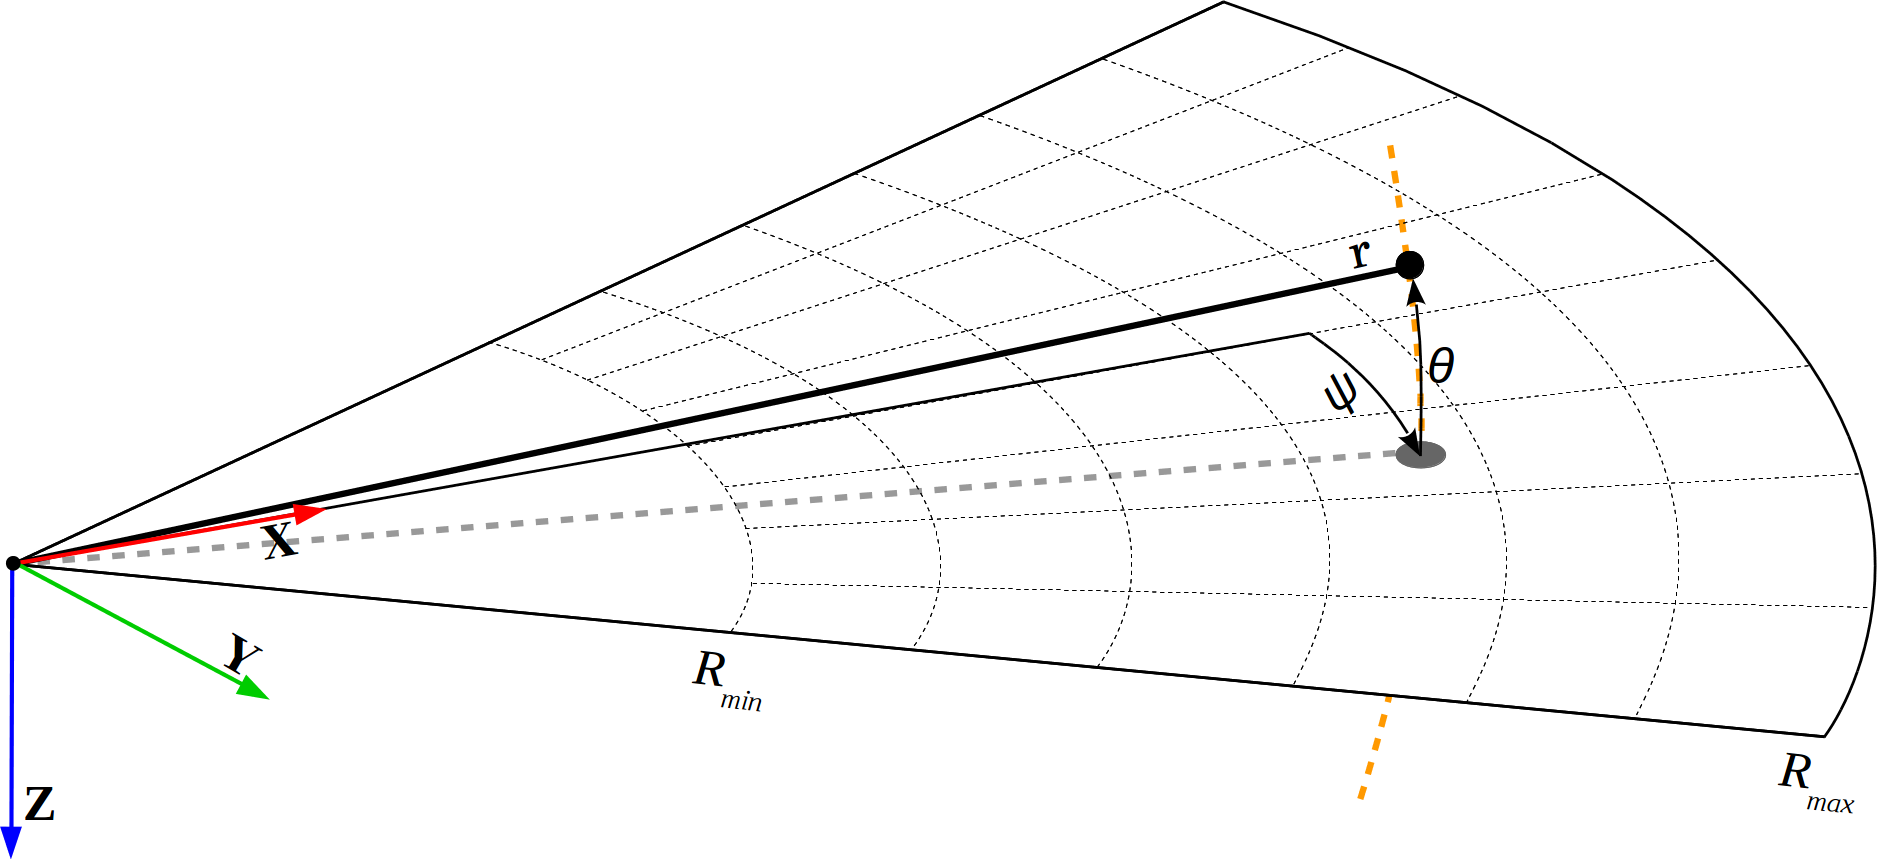
\includegraphics[width=\columnwidth]{figs/sonar_geometry_2}
    \captionsetup{justification=justified}
    \caption{Imaging sonar geometry. By the projection process, all 3D points  belonging to the same elevation arc (represented as dashed orange line) will be represented to the same image point in the 2D plane. Range $r$ and azimuth angle $\psi$ are measured, and elevation angle $\theta$ is lost. Sonar coverage area is defined by $R_{min}$ and $R_{max}$.}
    \label{fig:sonar_geometry}
\end{figure}

% ----------------------------------------------------------------------------------
\begin{figure*}[t]
    \centering
    \subfigure[][]{
    	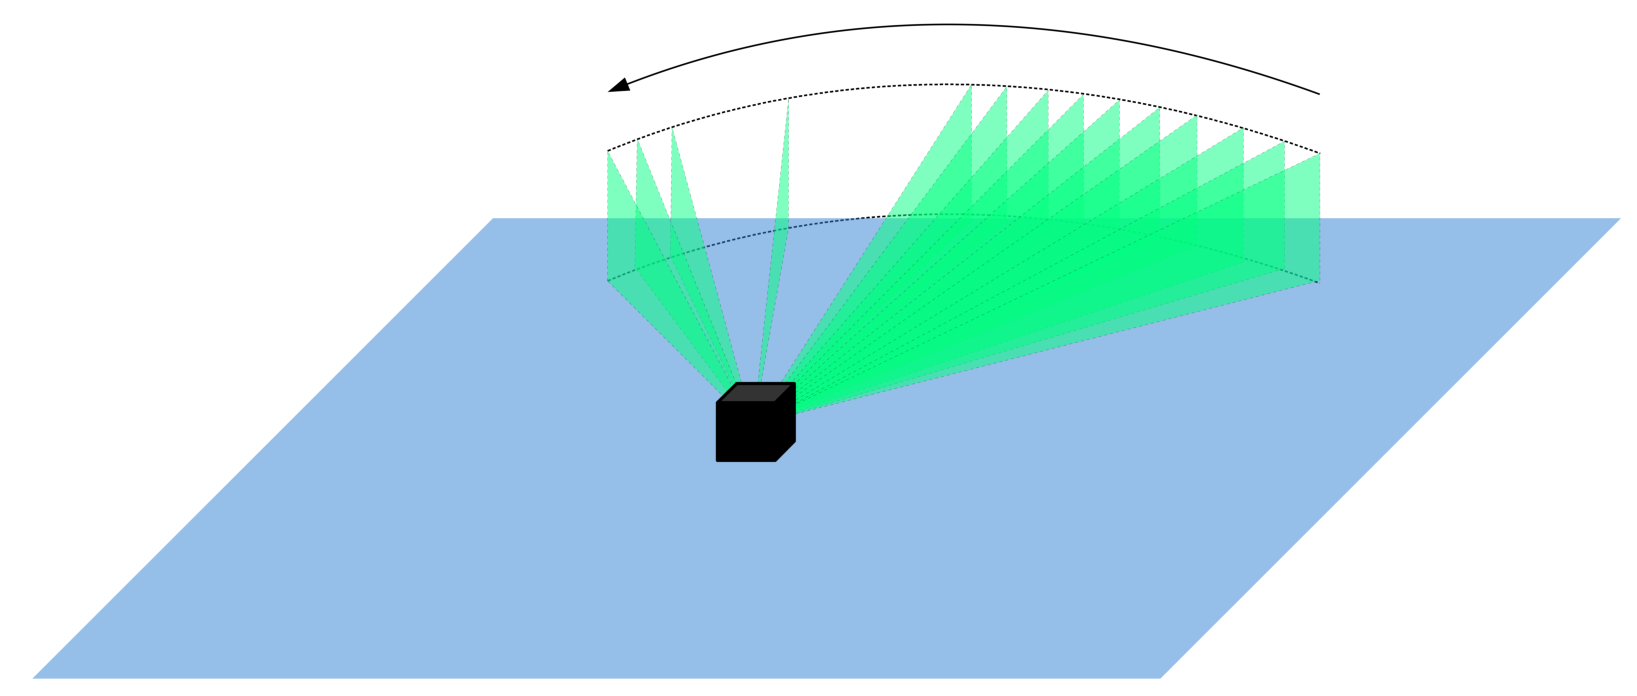
\includegraphics[width=\columnwidth]{figs/sonar_swarths_msis}
        \label{fig:swarths:msis}
    }
    \subfigure[][]{
    	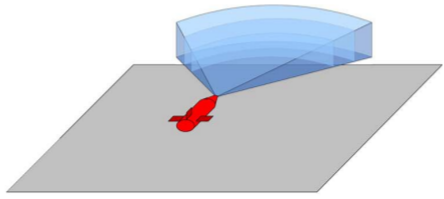
\includegraphics[width=\columnwidth]{figs/sonar_swarths_fls}
        \label{fig:swarths:fls}
    }
    \caption{Different underwater sonar readings: \subref{fig:swarths:msis}
    From a mechanical scanning imaging sonar and \subref{fig:swarths:fls}
    from a forward-looking sonar.}
    \captionsetup{justification=justified}
    \label{fig:sonar_devices}
\end{figure*}

% ----------------------------------------------------------------------------------

\subsection{Sonar characteristics}
\label{sonar:characteristics}

Although sonar devices overcome main limitations of optical sensors, they
present more difficult data interpretation due to:

\begin{enumerate}[a)]
    \item \textbf{Shadowing}: This effect is caused by objects blocking the
sound waves transmission, and causing regions behind them, without acoustic feedback. These regions are defined by a black spot in the sonar image, occluding part of the scene;
    \item \textbf{Non-uniform resolution}: The amount of pixels used to represent an echo intensity record in the Cartesian coordinate system grows as its range increases. This situation causes image distortions and object flatness;
    \item \textbf{Changes in viewpoint}: Imaging the same scene from different viewpoints can cause occlusions, shadows movements and significant  changes of observable objects \cite{hurtos2014}. For instance, when an    outstanding object is insonified, its shadow is shorter, as the sonar becomes closer;
    \item \textbf{Low signal-to-noise ratio (SNR)}: sonars suffer from low SNR mainly due the very-long-range scanning, and the presence of speckle noise introduced by acoustic wave interferences \cite{abbott1979};
    \item \textbf{Reverberation}: This phenomenon is caused when multiple acoustic waves, returning from the same object, are detected over the same ping, producing duplicated objects.
\end{enumerate}



% ----------------------------------------------------------------------------------

\subsection{Types of underwater sonar devices}
\label{sonar:devices}

The most common types of underwater acoustic sonars are MSIS and FLS. In
the former, the sonar image is built for each pulse, with one beam per
reading (see Fig. \ref{fig:swarths:msis}); the resulting sonar images in MSIS are usually depicted on a display pulse by pulse, and the head position reader is rotated according to motor step angle. After a full $360^{\circ}$ sector reading (or the desired sector defined by left and right limit angles), the accumulated sonar data is overwritten. The acquisition of a scanning image involves a relatively long time, introducing distortions caused by the vehicle movements. This sonar device is generally applied in obstacle avoidance \cite{ganesan2015} and navigation \cite{ribas2010} applications. As illustrated in Fig. \ref{fig:swarths:fls}, the whole forward view of an FLS is scanned and the current data is overwritten by the next scanning in a high frame rate, with all beams being read simultaneously; this is similar to a streaming video imagery for real-time applications; this imaging sonar is commonly used for navigation \cite{fallon2013}, mosaicing \cite{hurtos2014}, target tracking \cite{liu2016} and 3D reconstruction \cite{huang2015a}.

\begin{figure}[t]
    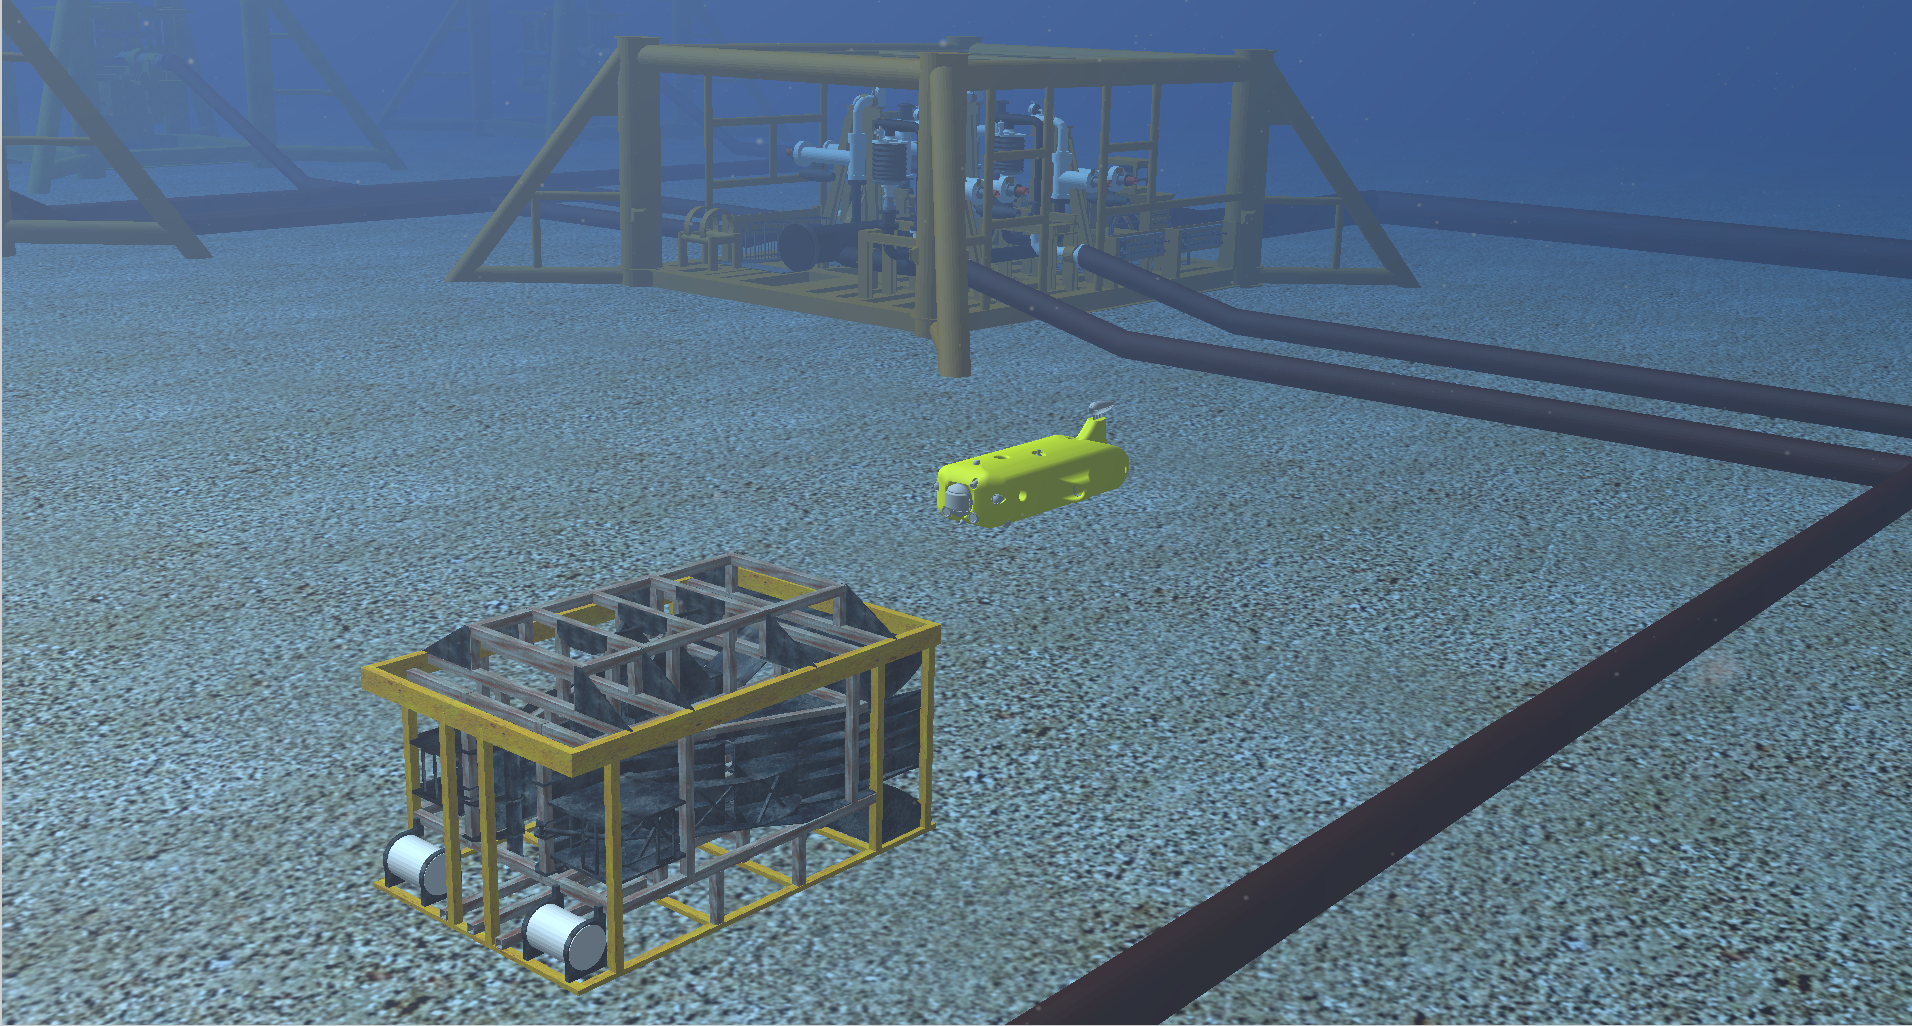
\includegraphics[width=\columnwidth]{figs/uwscene}
    \centering
    \captionsetup{justification=justified}
    \caption{The AUV in Rock-Gazebo underwater scene.}
    \label{fig:uwscene}
\end{figure}

% ----------------------------------------------------------------------------------

\begin{figure*}[t]
    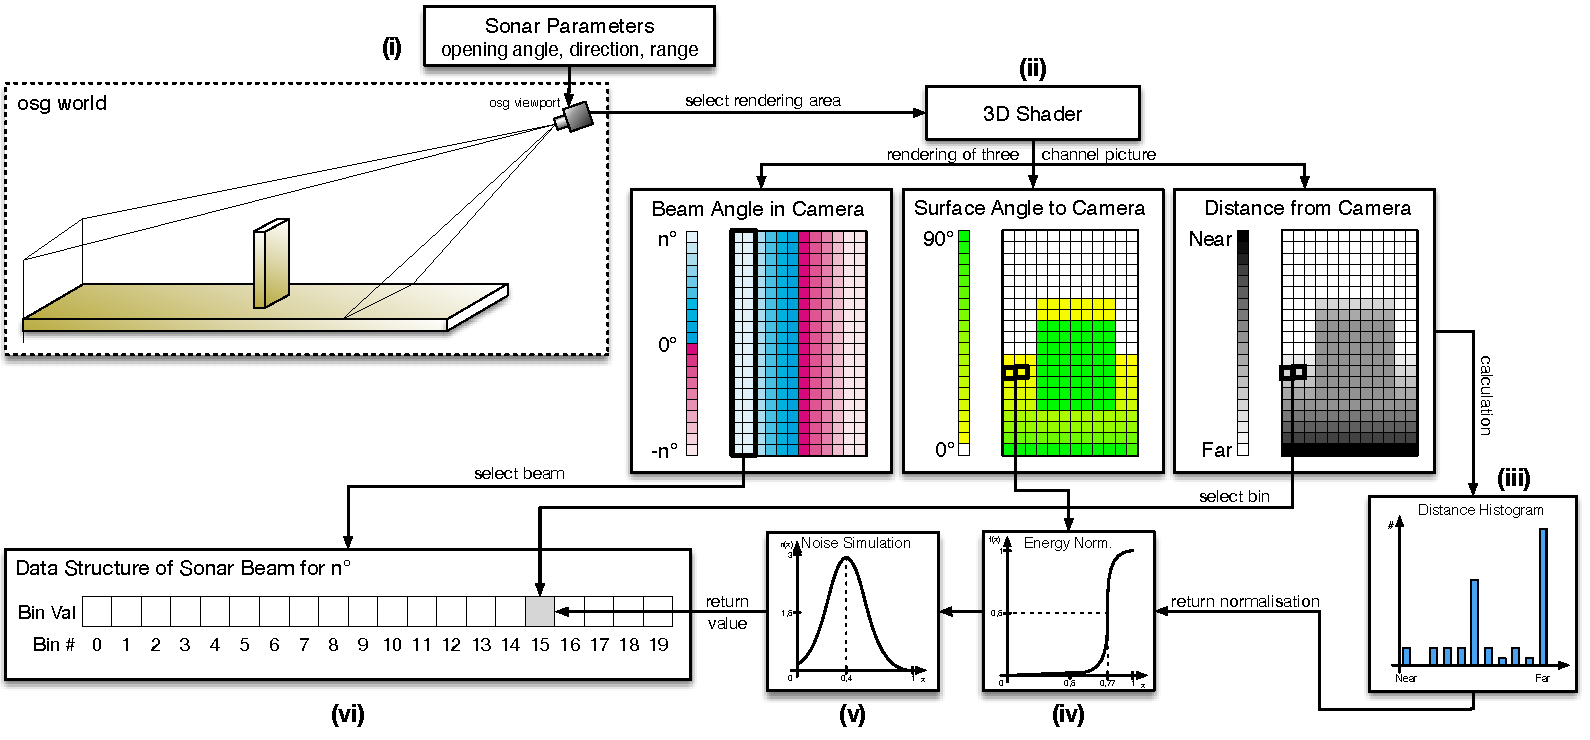
\includegraphics[width=0.85\paperwidth]{figs/sonar_sim}
    \centering
    \captionsetup{justification=justified}
    \caption{A graphical overview of the imaging sonar simulation process: (i) a virtual camera, specialized as the sonar device, samples the underwater scene; (ii) three 2D parameters are calculated by shader rendering on GPU: sonar field-of-view, echo intensity and pulse distance; the shader information is split into beam parts, according to the angle values, and the bin distance and echo intensity are defined by: (iii) distance histogram and (iv) energy normalization, respectively; (v) the speckle noise is applied to the final sonar data; (vi) and the simulated acoustic data is presented as Rock's data type.}
    \label{fig:sonar_sim}
\end{figure*}

% ----------------------------------------------------------------------------------

\section{GPU-based sonar simulation}
\label{dev}

The goal of our work is to simulate two types of underwater sonar with low computational cost. The complete pipeline of the proposed simulator (from the virtual scene to the simulated acoustic data) is detailed in the following sections. The sonar simulator is written in C++ with OpenCV \cite{bradski2000} support as Rock packages.

% ----------------------------------------------------------------------------------

\subsection{Rendering underwater scene}
\label{dev:uwscene}

In Rock-Gazebo framework \cite{watanabe2015}, Gazebo handles with physical forces, while Rock's visualization tools are responsible by the scene rendering. The graphical data in Rock are based on OpenSceneGraph framework, an open source C/C++ 3D graphics toolkit built on OpenGL. The osgOcean library is used to simulate the ocean visual effects. In our case, Rock-Gazebo integration provides the underwater scenario, allowing also real-time hardware-in-the-loop simulation with a virtual AUV.

%%%%Considerar tirar...
All scene aspects, such as world model, robot parts (including sensors and
joints) and other virtual objects are defined by simulation description files (SDF), which use the SDFormat \cite{sdformat2017}, an XML format used to describe simulated models and environments for Gazebo. Visual and collision geometries of vehicle and sensors are also described in specific file formats. Each component described in the SDF file becomes a Rock component, which is based on the Orocos real-time toolkit (RTT) \cite{soetens2005}, providing I/O ports, properties and operations as communication layers. When the models are loaded, Rock-Gazebo allows interaction between real world or simulated system components with the simulated models. A resulting scene sample of this integration is illustrated in Fig. \ref{fig:uwscene}.

% ----------------------------------------------------------------------------------

\subsection{Sonar rendering}
\label{dev:shader}

A rendering pipeline can be customized by defining GPU shaders. A shader is written in OpenGL Shading Language (GLSL) \cite{rost2009}, a high-level language with a C-based syntax, which enables more direct control of graphics pipeline, avoiding the use of low-level or hardware-specific languages. Shaders can describe the characteristics of either a vertex or a fragment (a single pixel). Vertex shaders are responsible by transforming the vertex position into a screen position by the rasterizer, generating texture coordinates for texturing, and lighting the vertex to determine each color. The rasterization results, in a set of pixels to be processed by fragment shaders, manipulate pixel location, depth and alpha values, and interpolated parameters from the previous stages, such as colors and textures.

In our work, the underwater scenes are sampled by a virtual camera (frame-by-frame), whose optical axis is aligned with the \textbf{opening angle}, the intended \textbf{viewing direction} and the coverage \textbf{range} of the simulated sonar device (see Fig. \ref{fig:sonar_sim}(i)). To reproduce the sonar imaging operation by using virtual camera frames, three parameters are computed in fragment and vertex shaders, during the rendering pipeline. This way, we are able to use the precomputed geometric information during the image rasterization process on GPU. The three parameters to render the sonar device using a virtual camera are illustrated in Fig. \ref{fig:sonar_sim}(ii), and are described as follows:

\begin{itemize}[]
    \item \textbf{Pulse distance} simulates the time of flight of the acoustic pulse, being calculated by the Euclidean distance between the camera center and the object surface;
    \item \textbf{Echo intensity} represents the energy reflection of the sound wave, calculated from the object surface normal regarding the camera;
    \item \textbf{Sonar field-of-view} is represented by the camera field-of-view in the horizontal direction.
\end{itemize}

By default, the shader encodes the raster data in 8-bit color channels for red, green, blue and alpha (RGBA). In our simulator, RGB channels are used to store the echo intensity, pulse distance and sonar field-of-view parameters to render the sonar from a virtual camera. The echo intensity parameter follows a real sonar common representation as 8-bit values. The pulse distance is replaced by the native GLSL 32-bit depth buffer to avoid precision limitation during the calculation of the distance histogram (see Fig. \ref{fig:sonar_sim}(iii)). As the field-of-view angle varies from the image center to both side directions, the sonar field-of-view is represented by 8-bit values without loss of precision. All of these three parameters are normalized into the interval [0,1]. For the echo intensity parameter, zero means no energy, while one means maximum echo energy. For pulse distance, the minimum value denotes a close object, while the maximum value represents a far one, limited by the sonar maximum range. Every sonar device has a maximum field-of-view; to represent this parameter in the rendering pipeline, the zero angle is in the center of the image, increasing until it reaches the half value of the maximum field-of-view of the simulated sonar device, for both sided borders; for example, if a sonar device has $120^{\circ}$ of field-of-view, the zero angle is in the center of the virtual camera, spanning $60^{\circ}$ to the right and $60^{\circ}$ to the left.

\begin{figure*}[!ht]
    \centering
    \setcounter{subfigure}{0}
    \subfigure[]{
        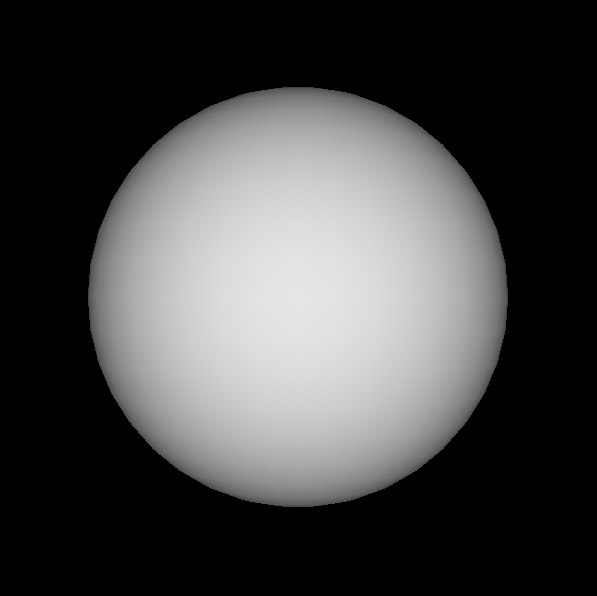
\includegraphics[width=0.25\paperwidth]{figs/normal_map_0}
        \label{fig:normal_0}
    }
    \setcounter{subfigure}{2}
    \subfigure[]{
        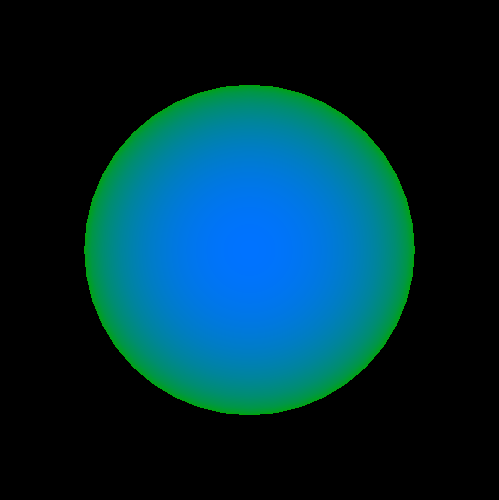
\includegraphics[width=0.25\paperwidth]{figs/normal_map_1}
        \label{fig:normal_1}
    }
    \setcounter{subfigure}{4}
    \subfigure[]{
        
\includegraphics[width=0.25\paperwidth]{figs/normal_map_2}
        \label{fig:normal_2}
    }
    \setcounter{subfigure}{1}
    \subfigure[]{
        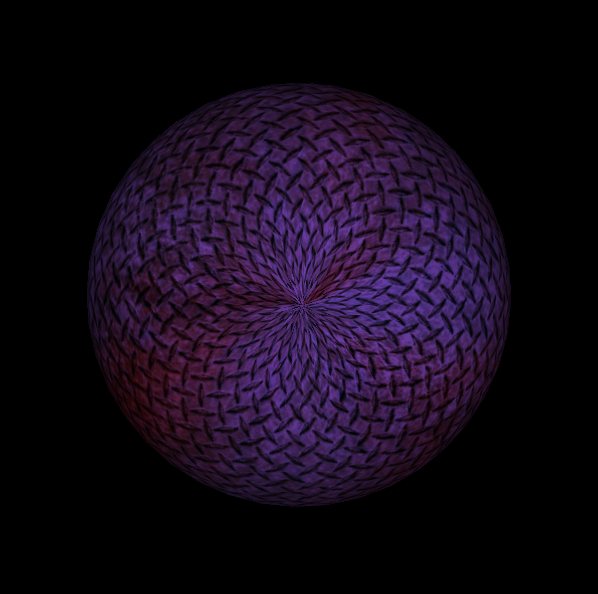
\includegraphics[width=0.25\paperwidth]{figs/normal_map_3}
        \label{fig:normal_3}
    }
    \setcounter{subfigure}{3}
    \subfigure[]{
        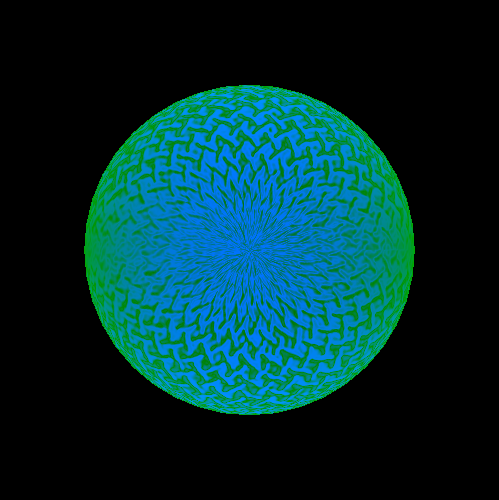
\includegraphics[width=0.25\paperwidth]{figs/normal_map_4}
        \label{fig:normal_4}
    }
    \setcounter{subfigure}{5}
    \subfigure[]{
        
\includegraphics[width=0.25\paperwidth]{figs/normal_map_5}
        \label{fig:normal_5}
    }
    \captionsetup{justification=justified}
    \caption{Example of shader rendering with normal mapping:
    A sphere without \subref{fig:normal_0} and with texture  \subref{fig:normal_3}; respective shader image representations of the spheres  in \subref{fig:normal_1} and \subref{fig:normal_4}, where the blue area represents the echo intensity parameter, while the green area means the pulse distance parameter. The final acoustic images are depicted in \subref{fig:normal_2} and \subref{fig:normal_5}. By using normal mapping technique, the textures changes the normal directions, and the sonar image details the appearance of object surface, like in real world sensing.}
    \label{fig:sonar_normal_mapping}
\end{figure*}

In real-world sensing, surfaces usually present irregularities
and different reflectance values. To render these surfaces in a virtual scene, the echo intensity values can also be defined by normal maps (see Fig. \ref{fig:sonar_normal_mapping}) and material property information (see Fig. \ref{fig:sonar_reflectances}). Normal mapping is a rendering technique, based on normal perturbation, that is used to simulate wrinkles and dents on the object surface by using RGB textures on shaders. This approach consumes less computational
resources for the same level of detail, compared with the displacement mapping
technique, because the geometry remains unchanged. Since normal maps are built in tangent space, interpolating the normal vertex and the texture, tangent, bi-tangent and normal (TBN) matrices are computed to convert the normal values into the world space. The visual differences of applying normal mapping in the actual scenes are illustrated in Figs. \ref{fig:normal_0} and \ref{fig:normal_1}; in the shader representation, in Figs. \ref{fig:normal_2} and \ref{fig:normal_3}; and the final sonar image, in Figs. \ref{fig:normal_4} and \ref{fig:normal_5}. The reflectance allows properly describing the intensity received back from observable objects in shader processing, according to the material
properties (for instance, aluminum has more reflectivity than wood and plastic).
When an object has the reflectivity property defined, the reflectance value
$\rho$ is passed to the fragment shader and processed on GPU. So, the final pixel intensity represents the product of surface normal angle by the reflectance value $\rho$. The reflectance affects the shader representation, as depicted in Figs. \ref{fig:reflectance:1}, \ref{fig:reflectance:0_35}, \ref{fig:reflectance:1_40} and \ref{fig:reflectance:2_12}), with a final sonar image shown in Figs. \ref{fig:reflectance:view:1}, \ref{fig:reflectance:view:0_35}, \ref{fig:reflectance:view:1_40} and \ref{fig:reflectance:view:2_12}.

\begin{figure}[!ht]
    \centering
    \setcounter{subfigure}{0}
    \subfigure[]{
    	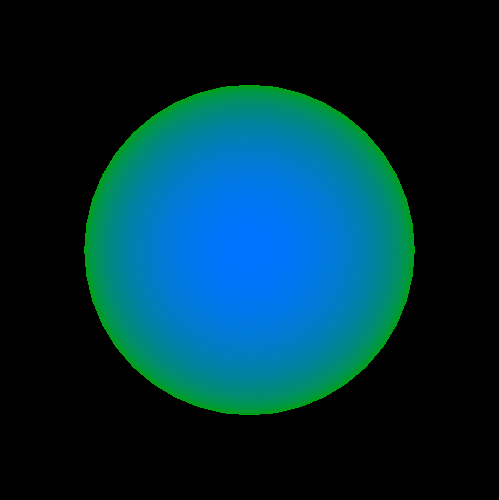
\includegraphics[width=0.45\columnwidth]{figs/reflectance_shader_1}
        \label{fig:reflectance:1}
    }
    \setcounter{subfigure}{4}
    \subfigure[]{
        
\includegraphics[width=0.45\columnwidth]{figs/reflectance_view_1}
        \label{fig:reflectance:view:1}
    }
    \setcounter{subfigure}{1}
    \subfigure[]{
    	
\includegraphics[width=0.45\columnwidth]{figs/reflectance_shader_0_35}
        \label{fig:reflectance:0_35}
    }
    \setcounter{subfigure}{5}
    \subfigure[]{
        
\includegraphics[width=0.45\columnwidth]{figs/reflectance_view_0_35}
        \label{fig:reflectance:view:0_35}
    }
    \setcounter{subfigure}{2}
    \subfigure[]{
    	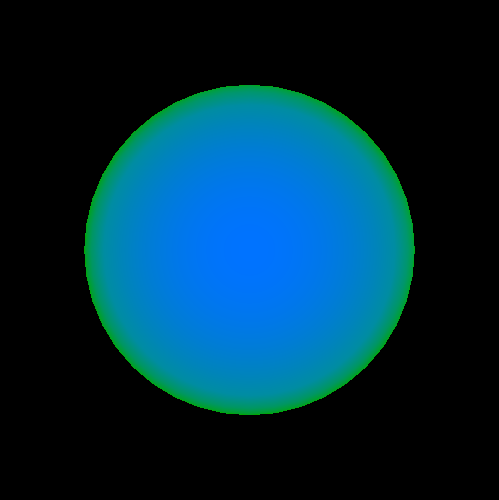
\includegraphics[width=0.45\columnwidth]{figs/reflectance_shader_1_40}
        \label{fig:reflectance:1_40}
    }
    \setcounter{subfigure}{6}
    \subfigure[]{
        
\includegraphics[width=0.45\columnwidth]{figs/reflectance_view_1_40}
        \label{fig:reflectance:view:1_40}
    }
    \setcounter{subfigure}{3}
    \subfigure[]{
    	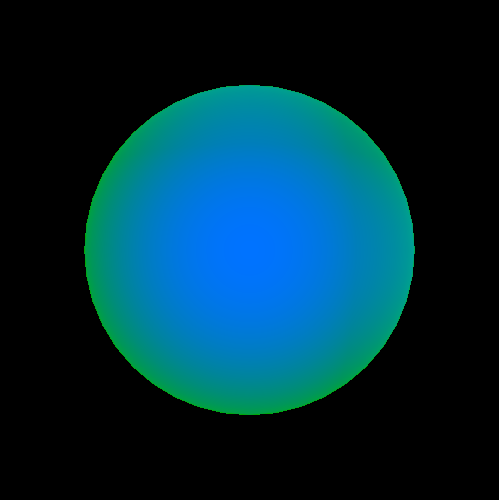
\includegraphics[width=0.45\columnwidth]{figs/reflectance_shader_2_12}
        \label{fig:reflectance:2_12}
    }
    \setcounter{subfigure}{7}
    \subfigure[]{
        
\includegraphics[width=0.45\columnwidth]{figs/reflectance_view_2_12}
        \label{fig:reflectance:view:2_12}
    }
    \captionsetup{justification=justified}
    \caption{Examples of different reflectance values, $\rho$, applied in
    shader image representation of the same target, where blue is the echo intensity parameter and green is the pulse distance parameter: \subref{fig:reflectance:1} raw image;
    \subref{fig:reflectance:0_35} $\rho = 0.35$;
    \subref{fig:reflectance:1_40} $\rho = 1.40$; and
    \subref{fig:reflectance:2_12} $\rho = 2.12$. The following
    acoustic images are presented in \subref{fig:reflectance:view:1},
    \subref{fig:reflectance:view:0_35}, \subref{fig:reflectance:view:1_40}
    and \subref{fig:reflectance:view:2_12}.}
    \label{fig:sonar_reflectances}
\end{figure}


% ----------------------------------------------------------------------------------
\subsection{Simulating operation of the sonar device}
\label{dev:sonardata}

The sonar rendering parameters are used to compute the corresponding acoustic representation. Since the sonar field-of-view is radially spaced over the horizontal field-of-view of the virtual camera (where all pixels in the same column have the same angle), the first step is to split the image into a number of beams (beamed sub-images). Each column of the sonar field-of-view parameter is related with a respective beam vector, according to sonar bearings, as illustrated in Fig. \ref{fig:sonar_sim}(vi).
In turn, one beam represents one or more columns. Each
beamed sub-image is converted into bin intensities using the pulse distance and the echo intensity parameters. In a real imaging sonar, the echo
measured back is sampled
over time, and the bin number is proportional to the sensor range. In other
words, the initial bins represent the closest distances, while the latest
bins represent the farthest ones. Therefore a distance histogram (see Fig. \ref{fig:sonar_sim}(iii)) is computed in order to
group the sub-image pixels with the respective bins, according to the pulse distance parameter and number of bins,
and calculate the accumulated intensity in each bin.

Due to the acoustic beam spreading and absorption in the water, the final
bins have less echo strength than the first ones. This is so, because the energy is
twice lost in the environment. To tackle with that issue, sonar devices
use an energy normalization based on time-varying gain for range dependence
compensation, which spreads losses in the bins. In our simulation approach,
the accumulated intensity, $I_{bin}$, in each bin (see Fig. \ref{fig:sonar_sim}(iv)) is normalized as

\begin{equation}
    \label{eq:1}
    I_{bin} = \sum\limits_{x=1}^N \frac{1}{N} \times S(i_{x}) \, ,
\end{equation}
where $x$ is the pixel location, $N$ is the distance histogram
value (number of pixels) of that bin, $S(i_{x})$ is a sigmoid function,
and $i_{x}$ is the echo intensity value of the pixel $x$. $\times$ defines an
element-wise multiplication.

Finally, the sonar image resolution must be big enough to contain all information of the bins. For that, the number of bins involved is directly proportional to the sonar image resolution.

% ----------------------------------------------------------------------------------
\subsubsection{Noise model}
\label{dev:noise}

Imaging sonar systems are disturbed by a multiplicative noise known as speckle,
which is caused by coherent processing of backscattered signals from multiple
distributed targets. This effect degrades image quality and visual evaluation. Speckle noise results in constructive and destructive interferences,
which are shown as bright and dark dots in the image. The noisy image has been
expressed, following \cite{lee1980}:

\begin{equation}
\label{eq:2}
y(t) = x(t) \times n(t) \, ,
\end{equation}
where $t$ is the time instant, $y(t)$ is the noised image, $x(t)$ is the
free-noise image, $n(t)$ is the speckle noise matrix, and $\times$ defines an
element-wise multiplication.

This type of noise is well-modeled as a Gaussian distribution. The physical explanation is provided by the central limit theorem, which states that the
sum of many independent and identically distributed random variables tends
to behave as a Gaussian random variable \cite{papoulis2002}. A Gaussian distribution is defined by following a non-uniform distribution, skewed towards low values, and applied as speckle noise in the simulated sonar image (see Fig. \ref{fig:sonar_sim}(v)). This noise simulation is repeated for each virtual acoustic frame.

%%%idem
\subsubsection{Integrating sonar device with Rock}
\label{dev:rock}

After the imaging sonar simulation process, from the virtual underwater scene to the representation of the degraded acoustic sonar data by noise, the resulting sonar data is encapsulated as Rock's sonar data type (see Fig. \ref{fig:sonar_sim}(vi)). This data type is provided as I/O port of a Rock's component, allowing the interaction with other simulated models and applications.

\begin{table}[t]
    \captionsetup{justification=justified}
    \caption{Sonar device configurations used on experimental evaluation.}
    \label{table:sonar_settings}
    \begin{center}
        \begin{tabular}{| c | c | c | c | c | c |}
            \hline
            \rule{0pt}{15pt}
            \makecell[c]{Device} & \makecell[c]{\shortstack{\# of\\ beams}} & \makecell[c]{\shortstack{\# of\\ bins}} & \makecell[c]{\shortstack{Field \\of view}} & \makecell[c]{\shortstack{Down\\tilt}} & \makecell{\shortstack{Motor\\Step}}\\
            \hline
            FLS  & 256 & 1000 & $120^{\circ}$ x $20^{\circ}$ & $20^{\circ}$  & - \\ \hline
            MSIS & 1   & 500  & $3^{\circ}$ x $35^{\circ}$	 & $0^{\circ}$  & $1.8^{\circ}$ \\ \hline
        \end{tabular}
    \end{center}
\end{table}

% ----------------------------------------------------------------------------------

\section{Simulation results and experimental analysis}
\label{results}

To evaluate our simulator, experiments were conducted by using a 3D model
of an AUV equipped with an MSIS and an FLS. Different scenarios were casted and studied, considering the sonar device configurations summarized in
Table \ref{table:sonar_settings}. In the experimental analysis, as the scene frames are being captured by
the sonars, the resulting acoustic images are sequentially presented,
on-the-fly (see Figs. \ref{fig:fls} and \ref{fig:msis}).

\begin{figure*}[!ht]
    \centering
    \setcounter{subfigure}{0}
    \subfigure[]{
        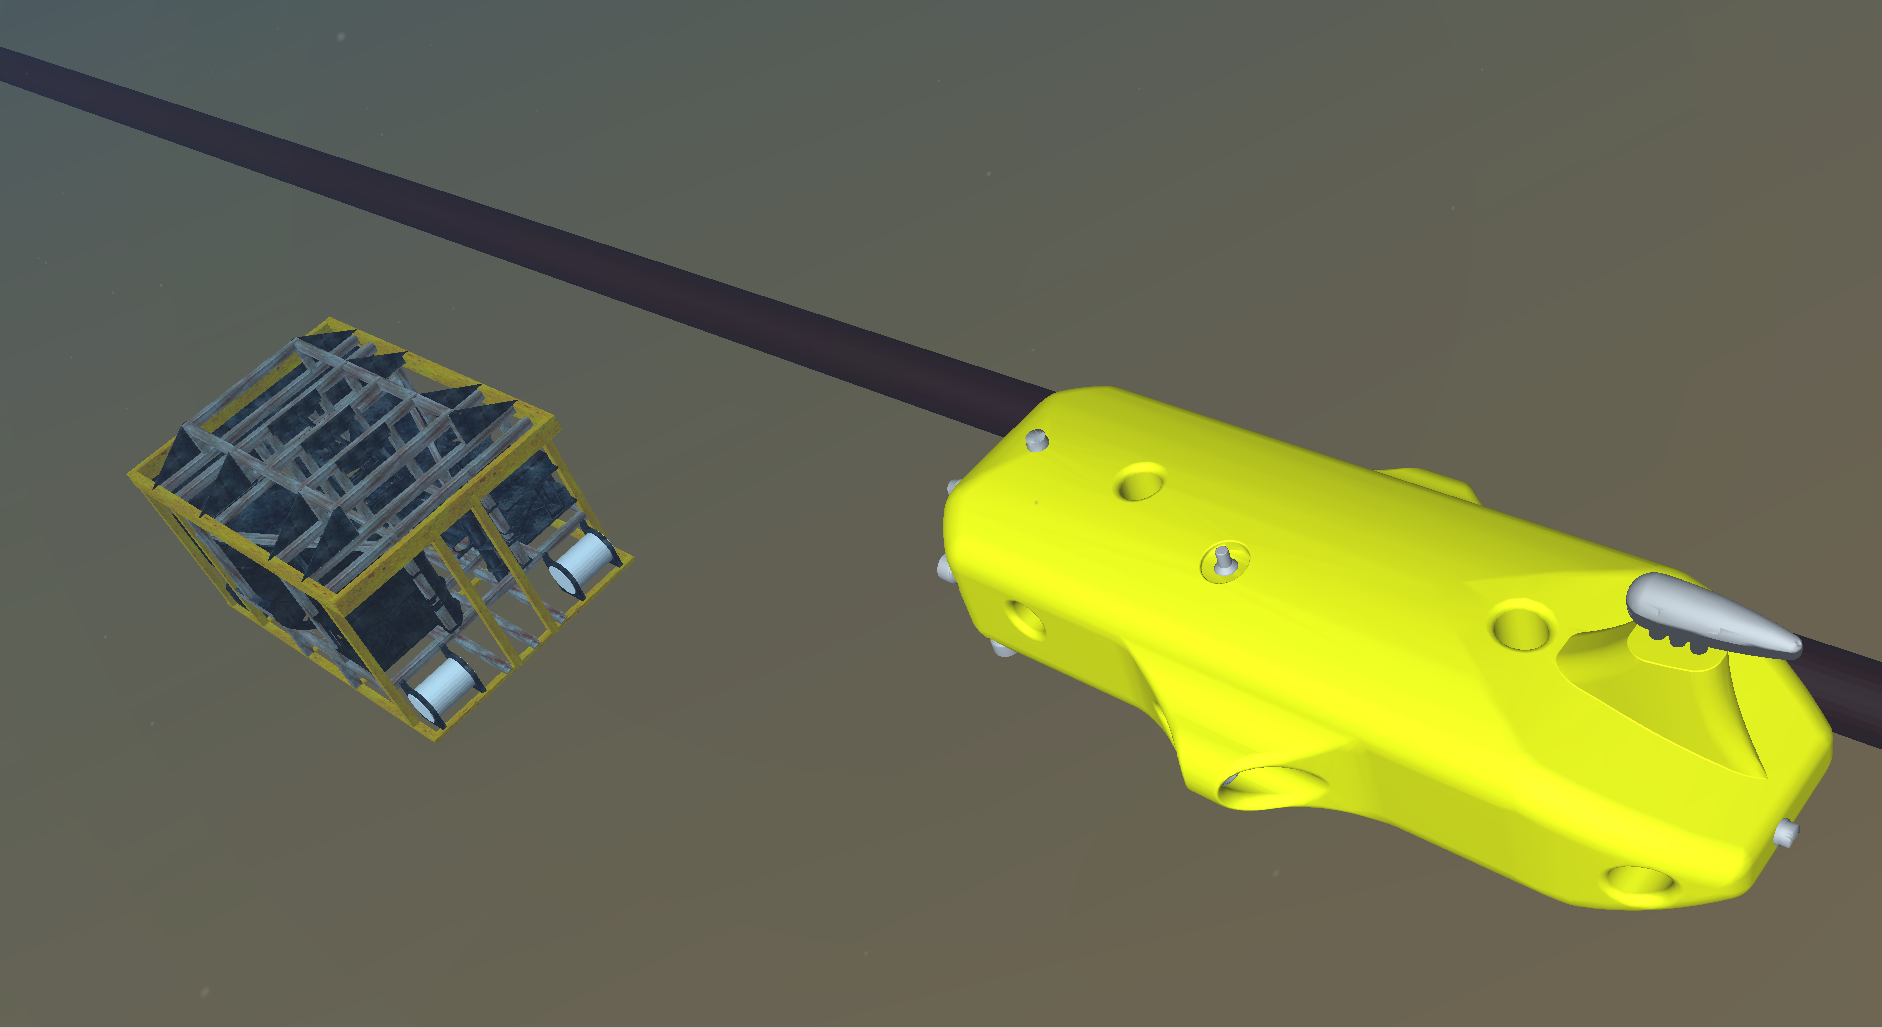
\includegraphics[width=0.4\paperwidth,height=6cm]{figs/fls_scene1}
        \label{fig:fls_scene1}
    }
    \setcounter{subfigure}{3}
    \subfigure[]{
        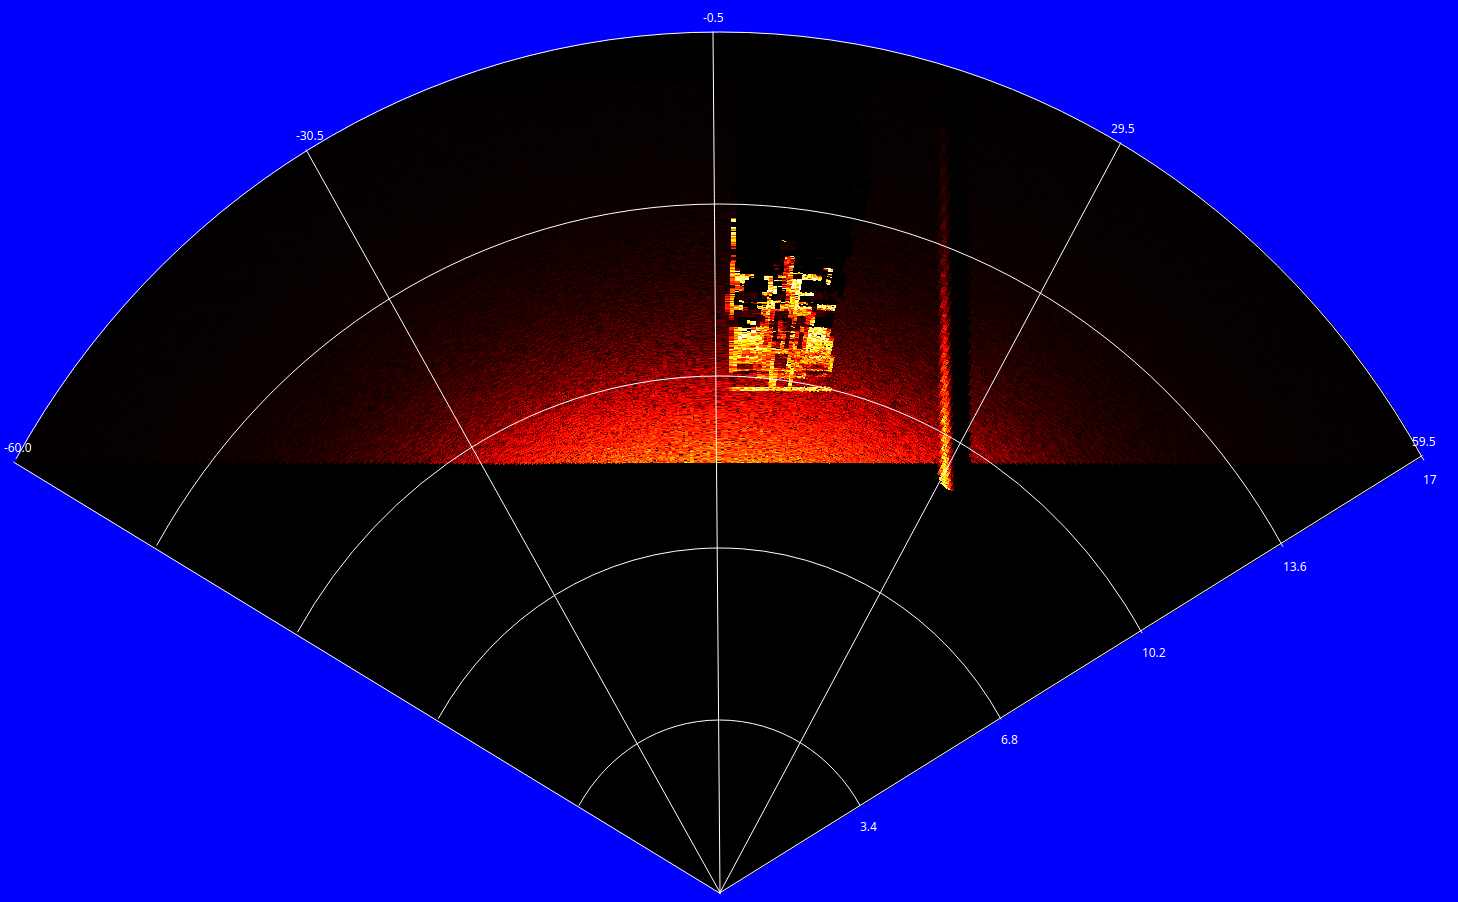
\includegraphics[width=0.4\paperwidth,height=6cm]{figs/fls_sim1}
        \label{fig:fls_sim1}
    }
    \setcounter{subfigure}{1}
    \subfigure[]{
        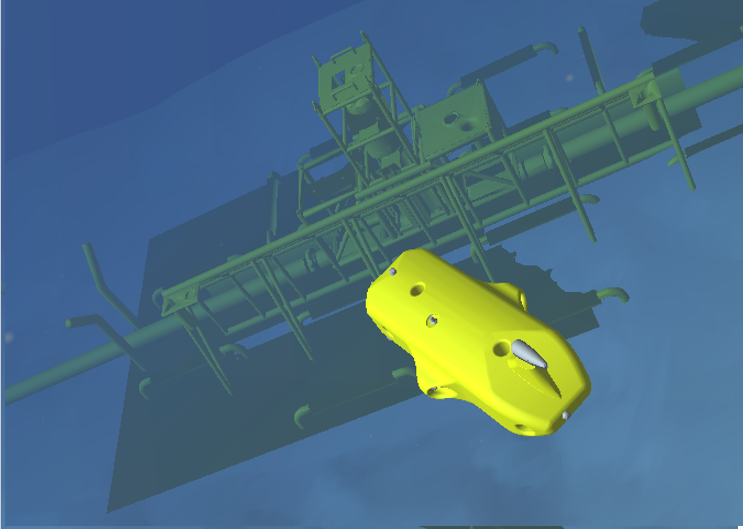
\includegraphics[width=0.4\paperwidth,height=6cm]{figs/fls_scene2}
        \label{fig:fls_scene2}
    }
    \setcounter{subfigure}{4}
    \subfigure[]{
        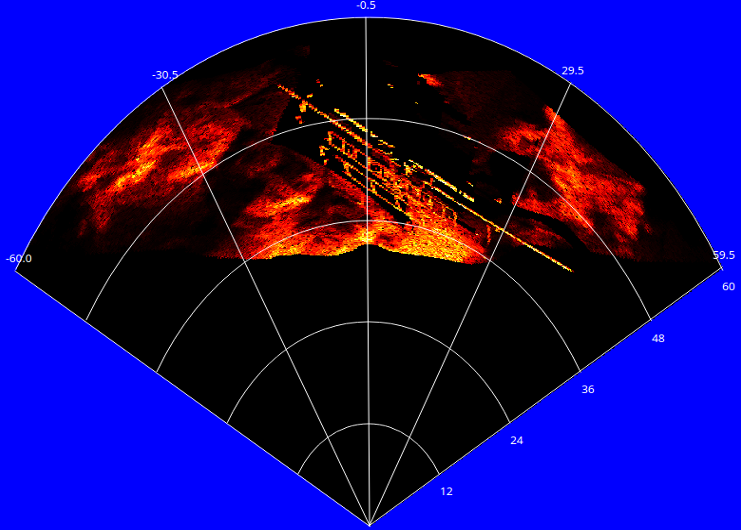
\includegraphics[width=0.4\paperwidth,height=6cm]{figs/fls_sim2}
        \label{fig:fls_sim2}
    }
    \setcounter{subfigure}{2}
    \subfigure[]{
        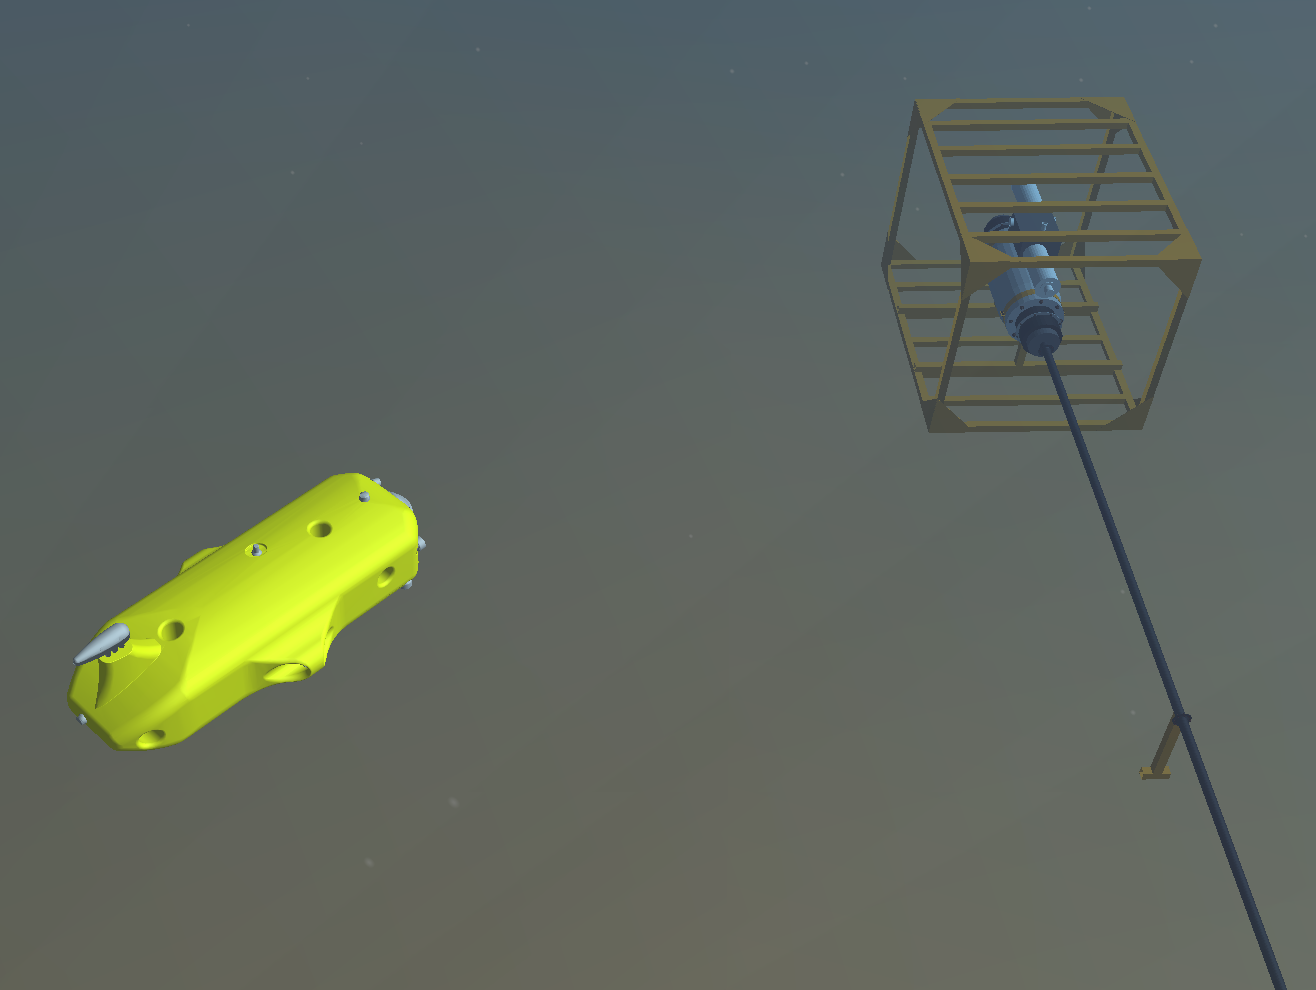
\includegraphics[width=0.4\paperwidth,height=6cm]{figs/fls_scene3}
        \label{fig:fls_scene3}
    }
    \setcounter{subfigure}{5}
    \subfigure[]{
        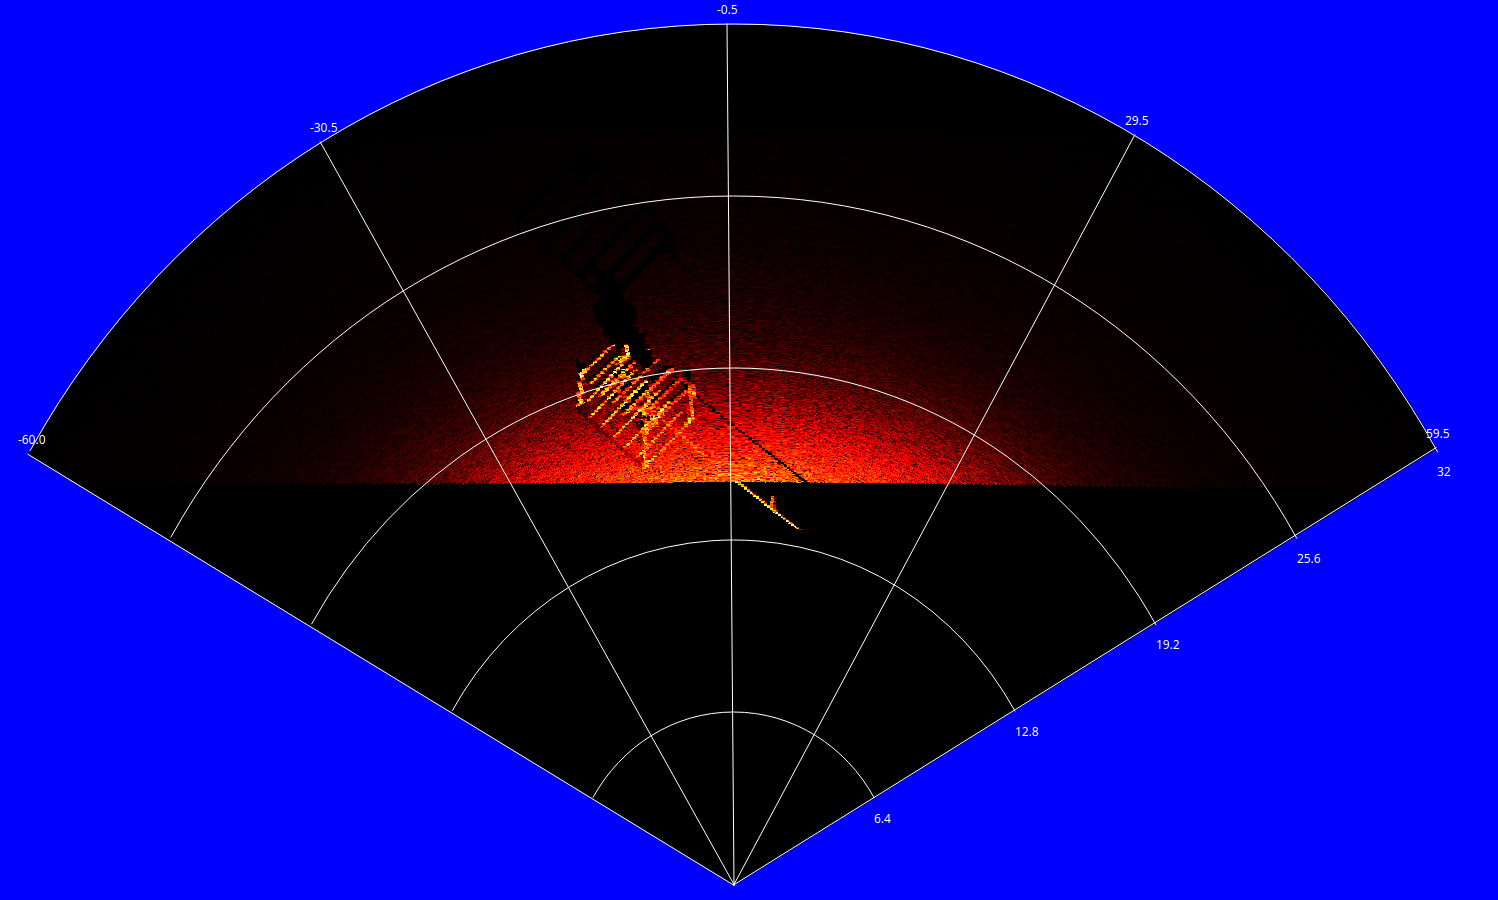
\includegraphics[width=0.4\paperwidth,height=6cm]{figs/fls_sim3}
        \label{fig:fls_sim3}
    }
    \captionsetup{justification=justified}
    \caption{Forward-looking sonar simulation experiments:
    \subref{fig:fls_scene1}, \subref{fig:fls_scene2} and \subref{fig:fls_scene3}
    present the virtual underwater trials, while \subref{fig:fls_sim1},
    \subref{fig:fls_sim2} and \subref{fig:fls_sim3} are the correspondent acoustic
    representations of each scenario, respectively.}
    \label{fig:fls}
\end{figure*}

\subsection{Experimental evaluation}

\begin{figure*}[!ht]
    \centering
    \setcounter{subfigure}{0}
    \subfigure[]{
        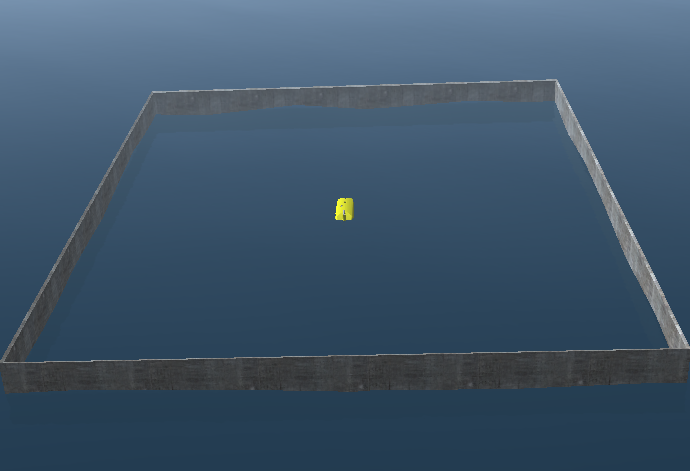
\includegraphics[width=0.4\paperwidth,height=6cm]{figs/msis_scene1}
        \label{fig:msis_scene1}
    }
    \setcounter{subfigure}{3}
    \subfigure[]{
        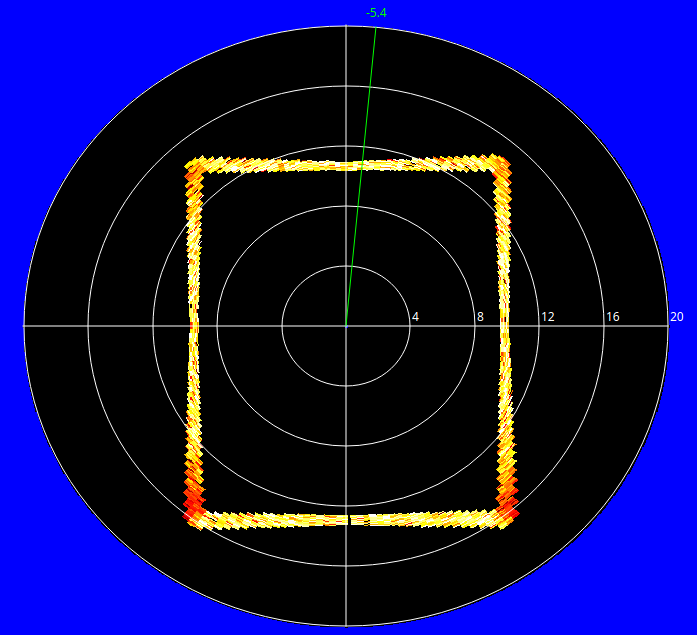
\includegraphics[width=0.4\paperwidth,height=6cm]{figs/msis_sim1}
        \label{fig:msis_sim1}
    }
    \setcounter{subfigure}{1}
    \subfigure[]{
        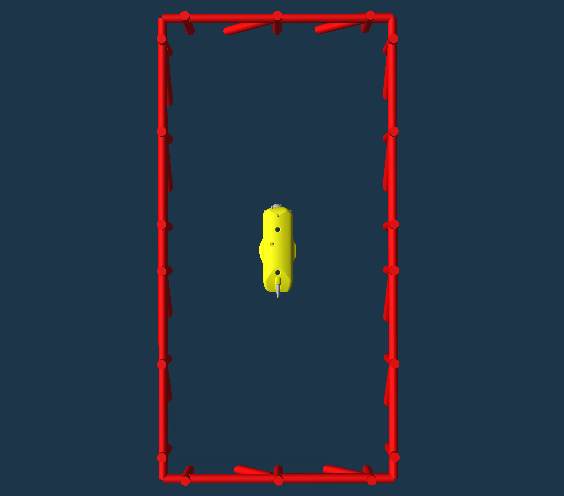
\includegraphics[width=0.4\paperwidth,height=6cm]{figs/msis_scene2}
        \label{fig:msis_scene2}
    }
    \setcounter{subfigure}{4}
    \subfigure[]{
        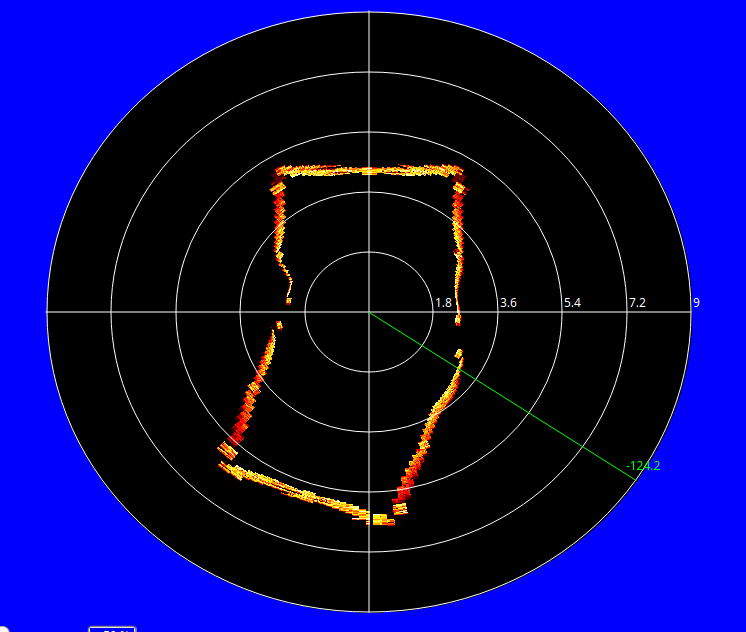
\includegraphics[width=0.4\paperwidth,height=6cm]{figs/msis_sim2}
        \label{fig:msis_sim2}
    }
    \setcounter{subfigure}{2}
    \subfigure[]{
        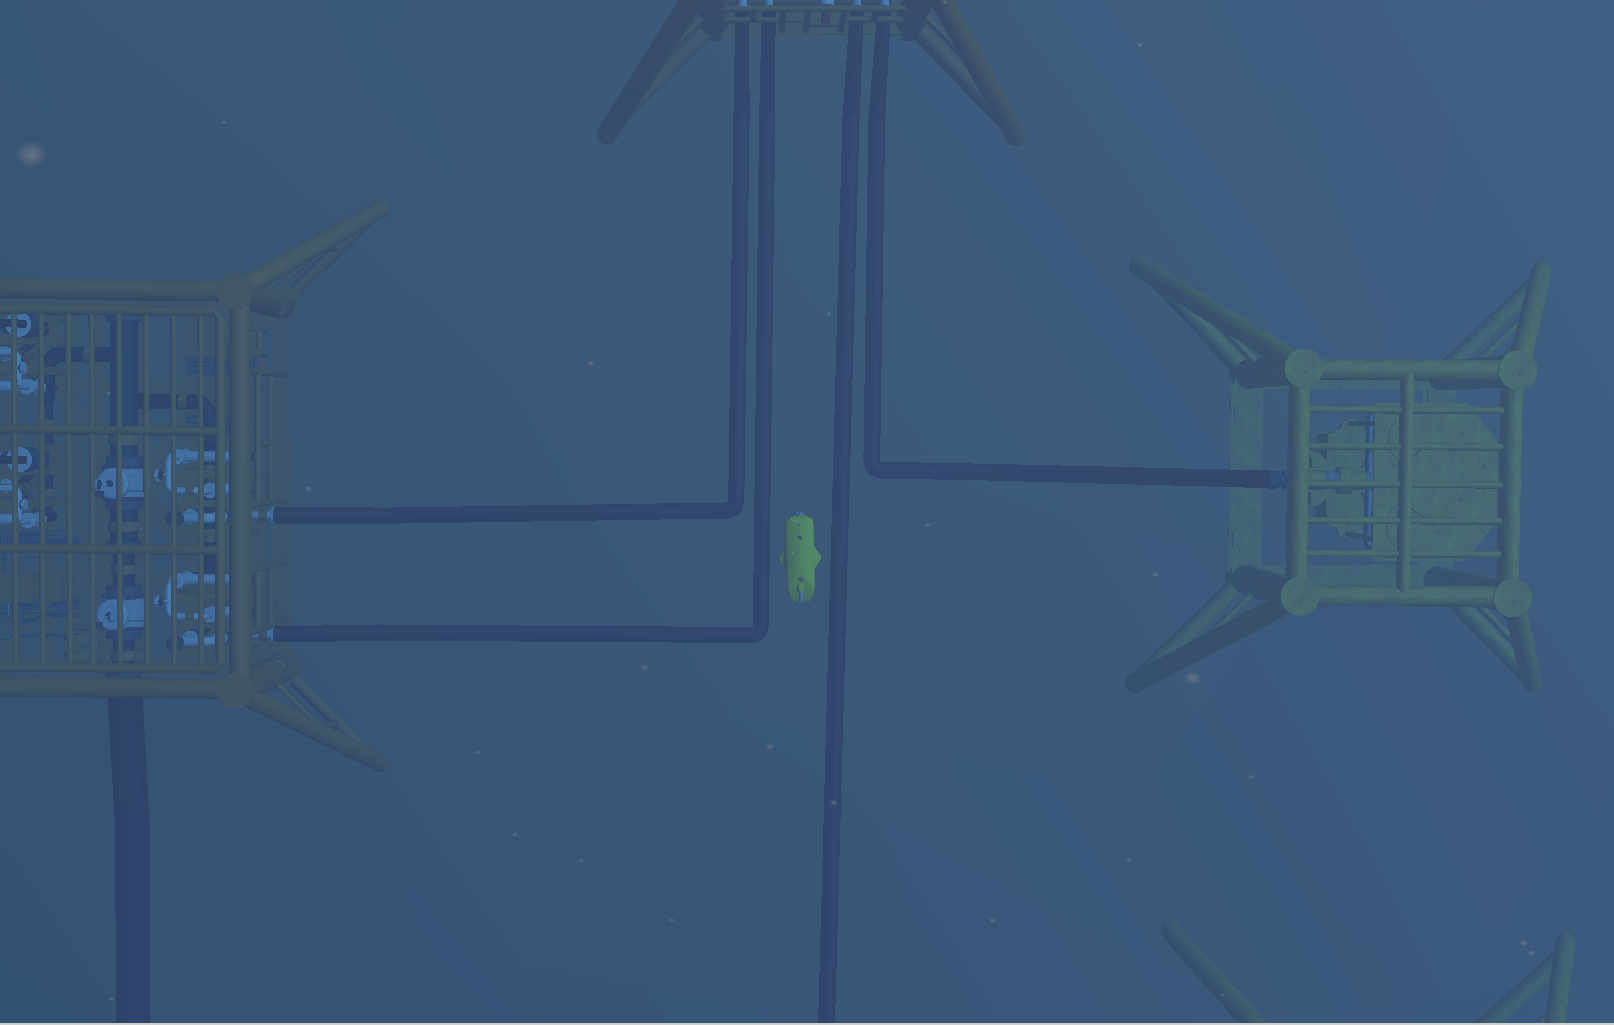
\includegraphics[width=0.4\paperwidth,height=6cm]{figs/msis_scene3}
        \label{fig:msis_scene3}
    }
    \setcounter{subfigure}{5}
    \subfigure[]{
        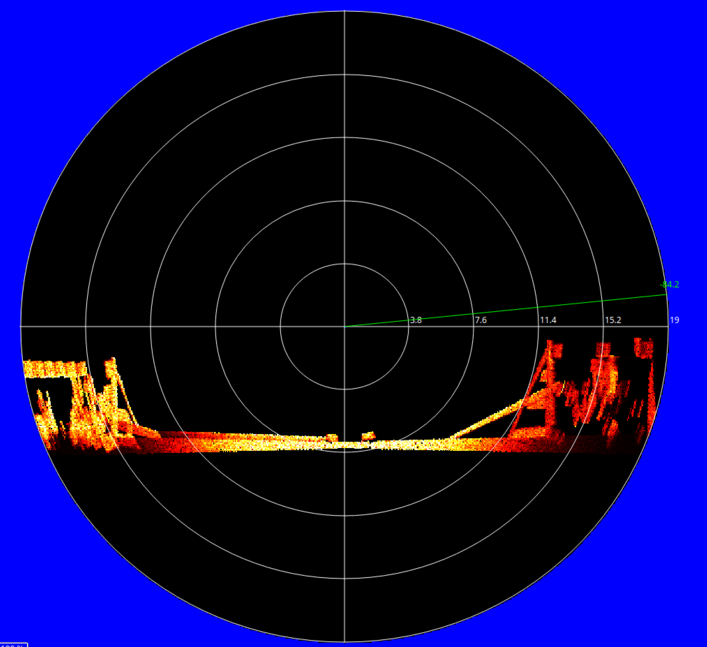
\includegraphics[width=0.4\paperwidth,height=6cm]{figs/msis_sim3}
        \label{fig:msis_sim3}
    }
    \captionsetup{justification=justified}
    \caption{Experiments using mechanical scanning imaging sonar in three
    different scenarios \subref{fig:msis_scene1}, \subref{fig:msis_scene2}
    and \subref{fig:msis_scene3}, and the respective processed simulated
    frames in horizontal orientation in \subref{fig:msis_sim1} and
    \subref{fig:msis_sim2}, and vertical orientation in \subref{fig:msis_sim3}.}
    \label{fig:msis}
\end{figure*}

\begin{table*}[t]
    \caption{Processing time to generate forward-looking sonar samples with different parameters.}
    \captionsetup{justification=justified}
    \label{table:fls}
    \begin{center}
        \begin{tabular}{| c | c | c | c | c | c | c |}
            \hline
            \# of samples & \# of beams & \# of bins & Field-of-view & Average time ($ms$) & Std dev ($ms$) & Frame rate ($fps$) \\
            \hline
            500     & 128     & 500       & $120^{\circ}$ x $20^{\circ}$        & 54.7    & 3.7   & 18.3 \\ \hline
            500     & 128     & 1000      & $120^{\circ}$ x $20^{\circ}$        & 72.3	& 8.9   & 13.8 \\ \hline
            500     & 256     & 500       & $120^{\circ}$ x $20^{\circ}$        & 198.7	& 17.1  & 5.0  \\ \hline
            500     & 256     & 1000      & $120^{\circ}$ x $20^{\circ}$        & 218.2	& 11.9  & 4.6  \\ \hline
            500     & 128     & 500       & $90^{\circ}$ x $15^{\circ}$         & 77.4	& 11.8  & 12.9 \\ \hline
            500     & 128     & 1000      & $90^{\circ}$ x $15^{\circ}$         & 94.6	& 10.2  & 10.6 \\ \hline
            500     & 256     & 500       & $90^{\circ}$ x $15^{\circ}$         & 260.8	& 18.5  & 3.8  \\ \hline
            500     & 256     & 1000      & $90^{\circ}$ x $15^{\circ}$         & 268.7	& 16.7  & 3.7  \\ \hline
        \end{tabular}
    \end{center}
\end{table*}

\begin{table*}
    \caption{Processing time to generate mechanical scanning imaging sonar samples with different parameters.}
    \captionsetup{justification=justified}
    \label{table:msis}
    \begin{center}
        \begin{tabular}{| c | c | c | c | c | c |}
            \hline
            \# of samples & \# of bins & Field-of-view & Average time ($ms$) & Std dev ($ms$) & Frame rate ($fps$) \\
            \hline
            500     & 500       & $3^{\circ}$ x $35^{\circ}$        & 8.8	    & 0.7  & 113.4 \\ \hline
            500     & 1000      & $3^{\circ}$ x $35^{\circ}$        & 34.5	& 1.6  & 29.0  \\ \hline
            500     & 500       & $2^{\circ}$ x $20^{\circ}$        & 10.3	& 0.6  & 96.7  \\ \hline
            500     & 1000      & $2^{\circ}$ x $20^{\circ}$        & 41.7	& 3.7  & 24.0  \\ \hline
        \end{tabular}
    \end{center}
\end{table*}


The virtual FLS from AUV was used to insonify the scenes from three distinct
scenarios. A docking station, in parallel with a pipeline on the seabed,
composes \textbf{the first scenario} (see Fig. \ref{fig:fls_scene1}); the
target surface is well-defined in the simulated acoustic frame (see
Fig. \ref{fig:fls_sim1}), as well as the shadows and speckle noise; given that the docking station is metal-made, the texture and reflectivity were set such
that a higher intensity shape was resulted in comparison with the other observable targets.
\textbf{The second scenario} presents the vehicle in front of a manifold model
in a non-uniform seabed (see Fig. \ref{fig:fls_scene2}); the target model was
insonified to generate the sonar frame from the underwater scene (see Fig. \ref{fig:fls_sim2}); the frontal
face of the target, as well the portion of the seabed and the degraded data
by noise, are clearly visible in the FLS image; also, a long acoustic shadow
is formed behind the manifold, occluding part of the scene. \textbf{The
third scenario} contains a sub-sea isolation valve (SSIV) structure, connected
to a pipeline in the bottom (see Fig. \ref{fig:fls_scene3}); the simulated
acoustic image, depicted in Fig. \ref{fig:fls_sim3}, also present shadows,
material properties and speckle noise effects. Due to sensor configuration and
robot position, the initial bins usually present a blind region in the three
simulated scenes, caused by absence of objects at lower ranges, similar to real
sonar images. It is noteworthy that the brightness of sea-floor decreases as it is
farther from sonar, because of the normal orientation of the surface.

The MSIS was also simulated in three different experiments. The robot in a
big textured tank composes \textbf{the first scene} (see Fig.
\ref{fig:msis_scene1}); similar to the first scenario of FLS experiment,
the reflectivity and texture were set to the target; the rotation of the
sonar head position, by a complete $360^{\circ}$ scanning, produced the acoustic
frame of tank walls (see Fig. \ref{fig:msis_sim1}). \textbf{The second scene}
involves the vehicle's movement during the data acquisition process; the scene
contains a grid around the AUV (see Fig. \ref{fig:msis_scene2}), captured by a front MSIS mounted horizontally; this trial induces a distortion in the final
acoustic frame, because the relative sensor position with respect to the
surrounding object changes, as the sonar image is being built (see
Fig. \ref{fig:msis_sim2}); in this case, the robot rotates $20^{\circ}$ left
during the scanning. \textbf{The last scene} presents the AUV over oil
and gas structures on the sea bottom (see Fig. \ref{fig:msis_scene3});
using an MSIS located in the back of the AUV with a vertical orientation, the scene was scanned to produce the acoustic visualization; as illustrated in Fig. \ref{fig:msis_sim3}, object surfaces present clear definition in the slice scanning of the sea-floor.

All the experimental scenarios was defined in order to provide enough variability of specific phenomena usually found in real sonar images, such as acoustic shadows, noise interference, surface irregularities and properties, distortion during the acquisition process and changes of acoustic intensities. However, the speckle noise application is restricted to regions with acoustic intensity, as shown in Figs. \ref{fig:fls_sim3} and \ref{fig:msis_sim1}. This fact is due to our sonar model be multiplicative (defined in Eq. \ref{eq:2}). In real sonar images, the noise also granulates the shadows and blind regions. The sonar simulator can be improved by inserting an additive noise to our model.
The impact of incorporating additive noise on the image is more severe than that of multiplicative, and we decided to collect more data before including a specific additive noise in our simulator, at this moment. A second feature missing in our simulated acoustic images are the ghost effects caused by reverberation. This lacking part can be addressed by implementation of a multi-path propagation model \cite{huang2015b}, where the signal propagates along several different paths, resulting in fading and reverberation effects. Simulating the multi-path reflection is computationally costly, thus we need more time to model and include the reverberation phenomenon, considering the real-time constraints.

\begin{figure*}[!ht]
    \centering
    \setcounter{subfigure}{0}
    \subfigure[]{
        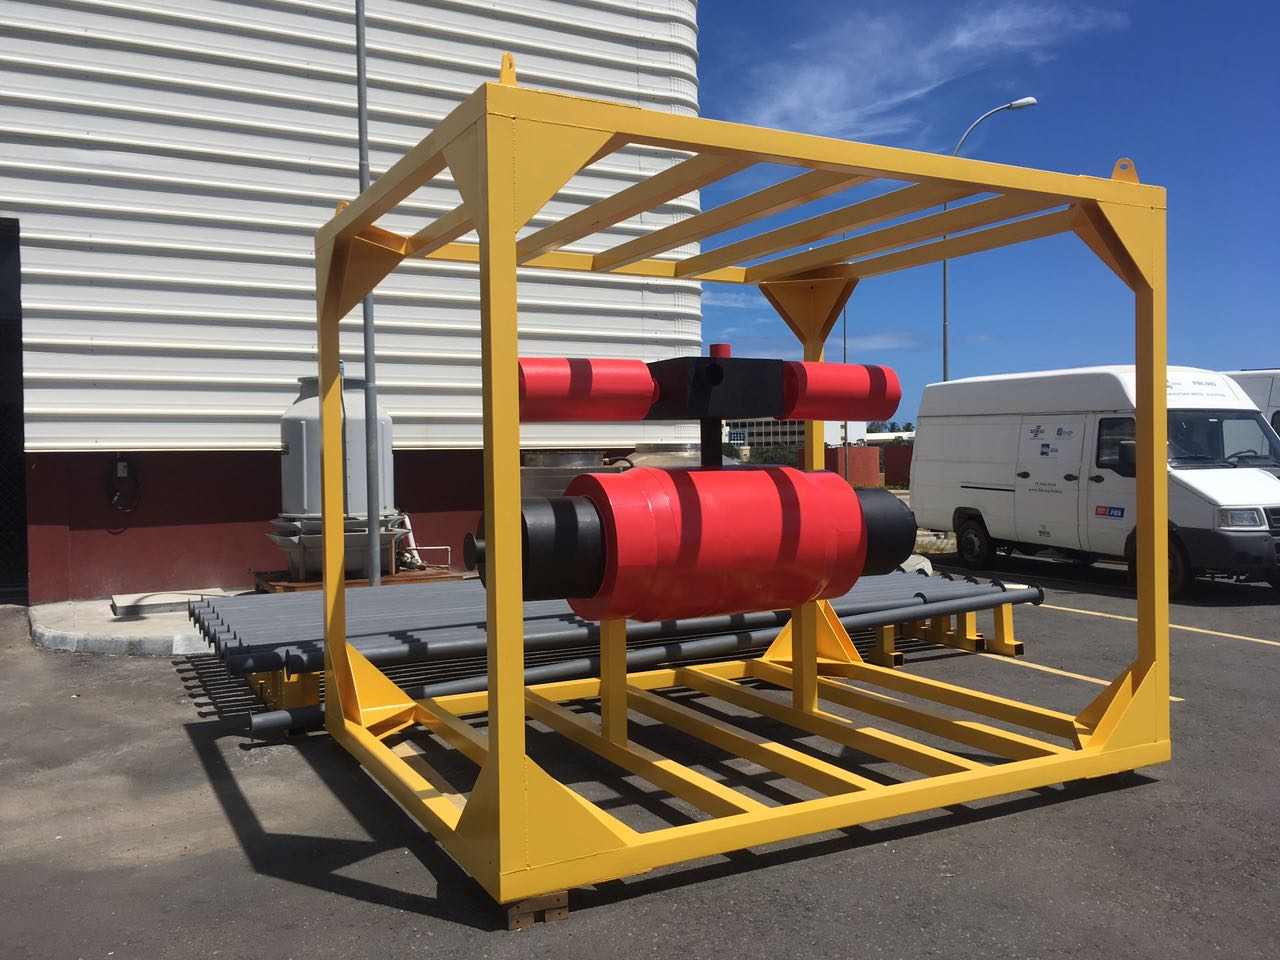
\includegraphics[width=0.4\paperwidth,height=6cm]{figs/eval_ssiv_photo}
        \label{fig:eval:ssiv:photo}
    }
    \setcounter{subfigure}{3}
    \subfigure[]{
        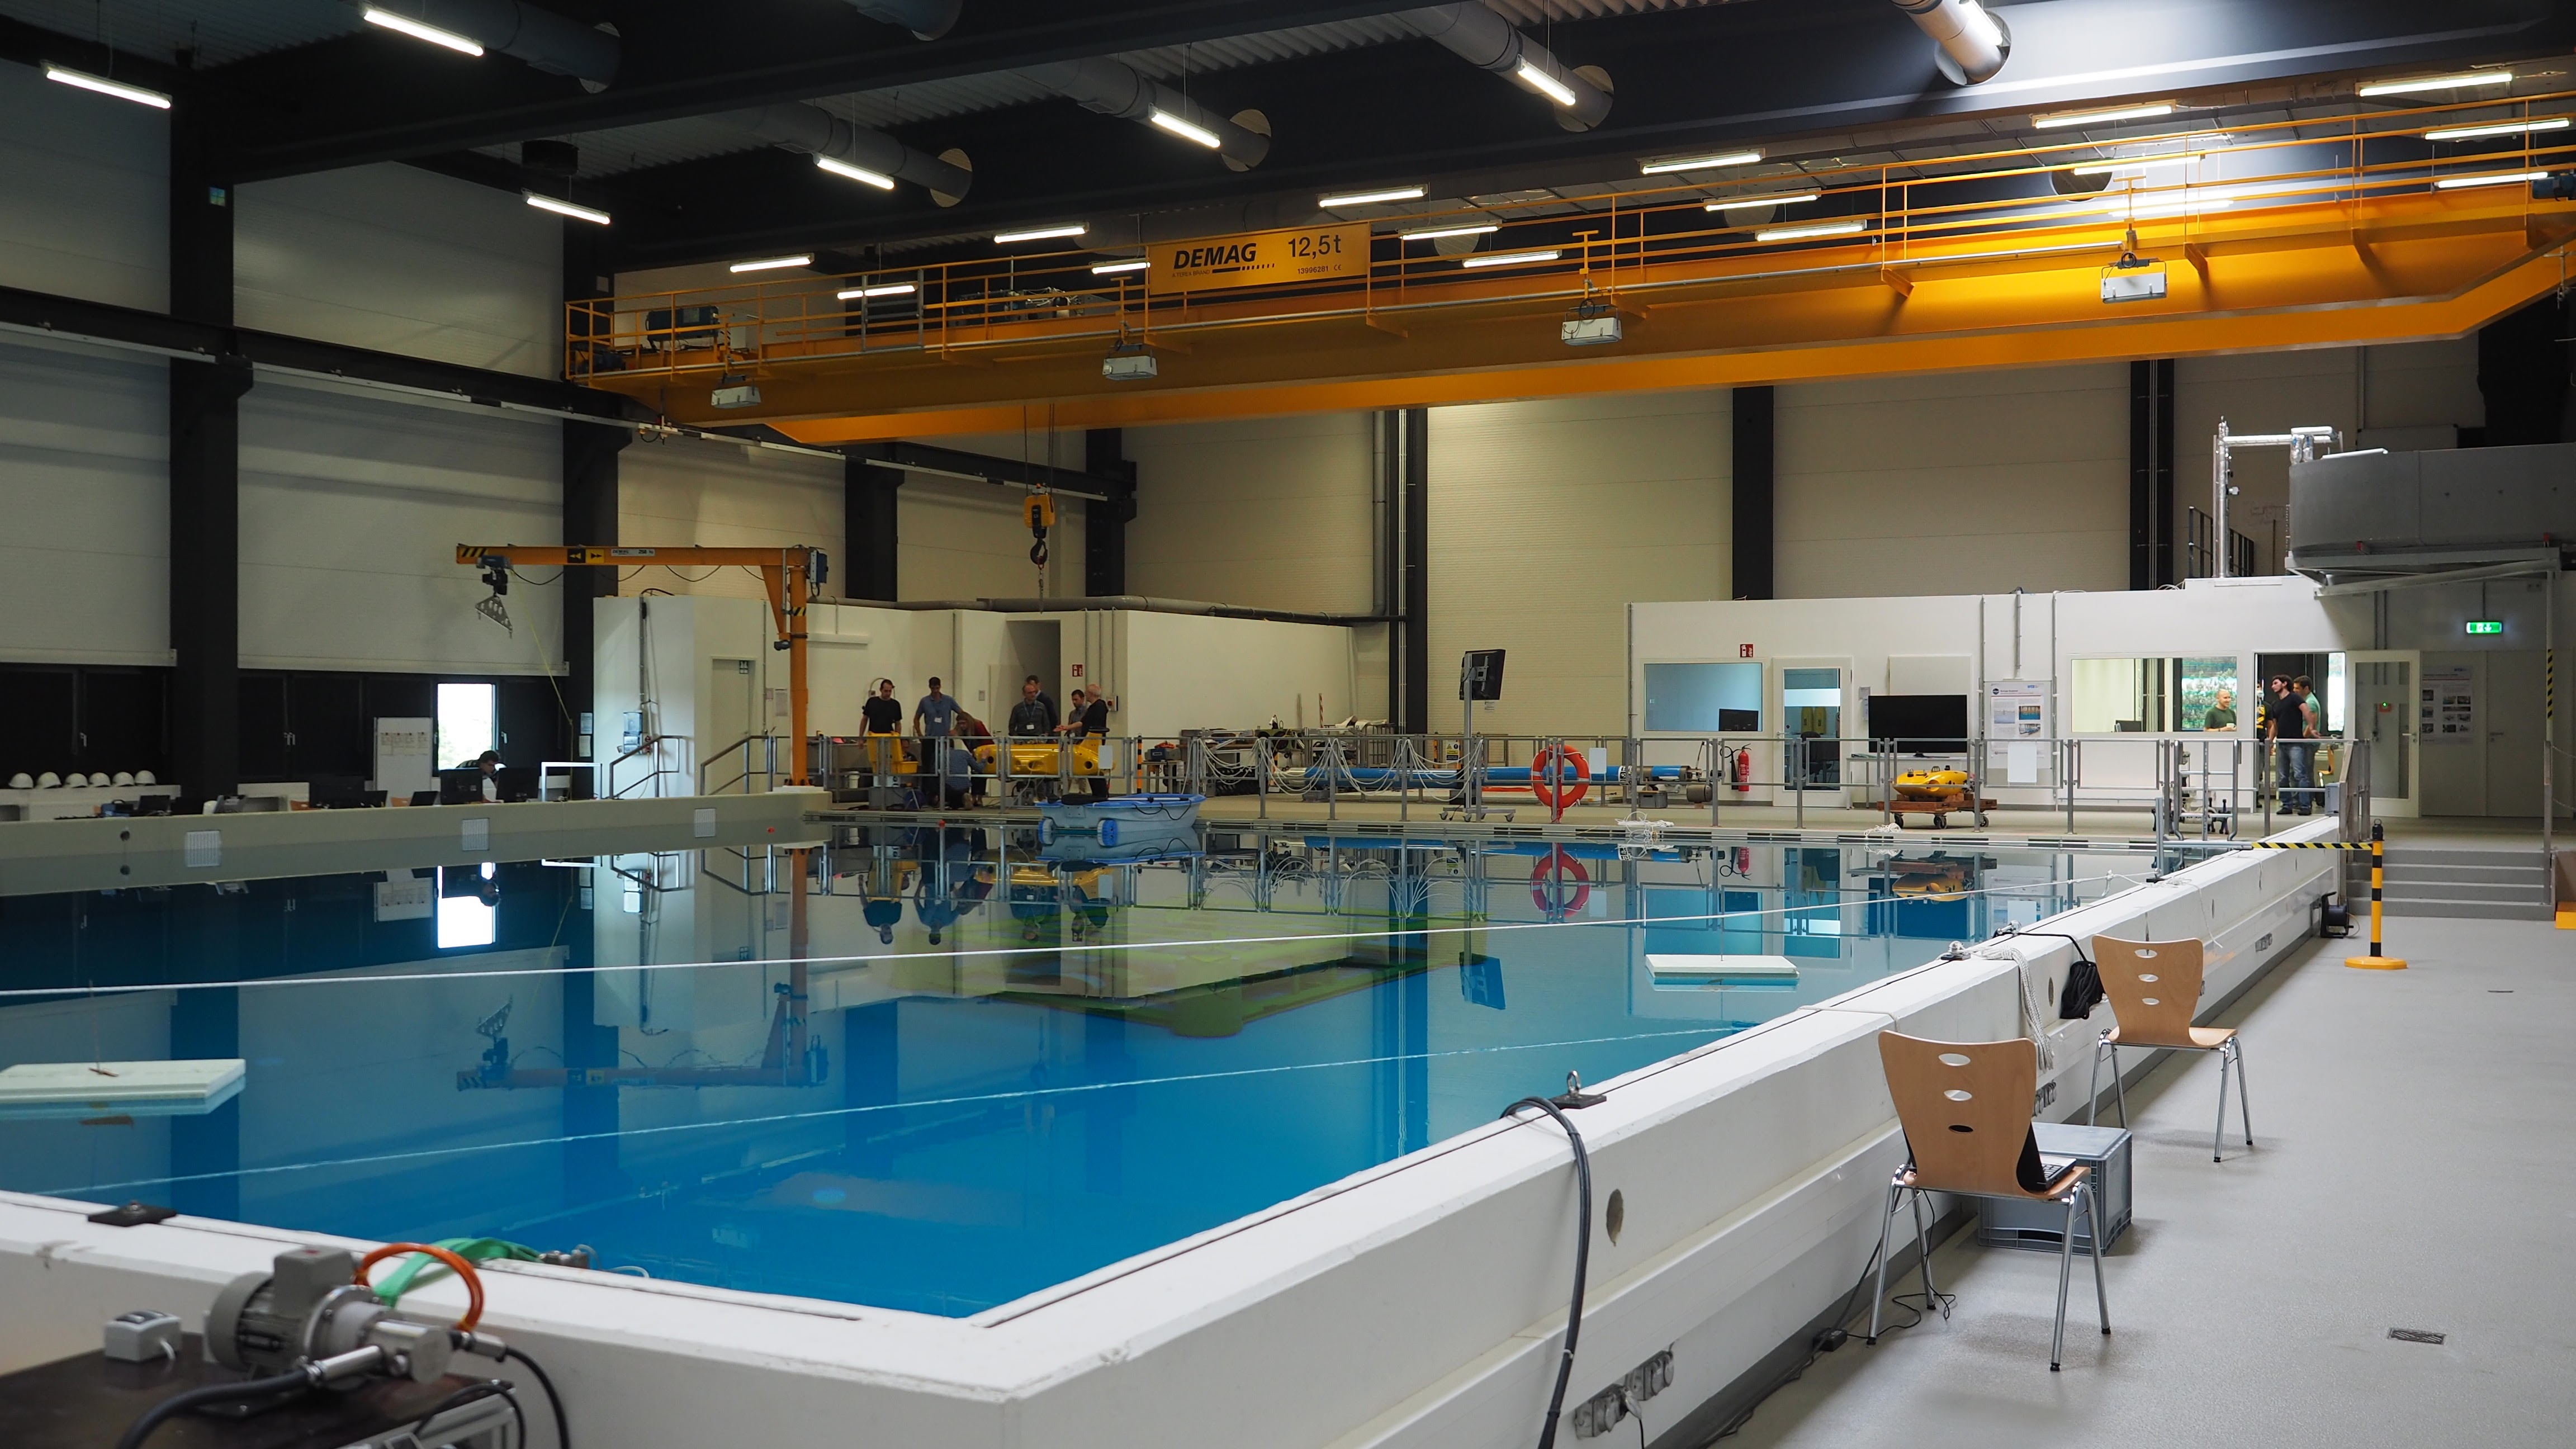
\includegraphics[width=0.4\paperwidth,height=6cm]{figs/eval_tank_photo}
        \label{fig:eval:tank:photo}
    }
    \setcounter{subfigure}{1}
    \subfigure[]{
        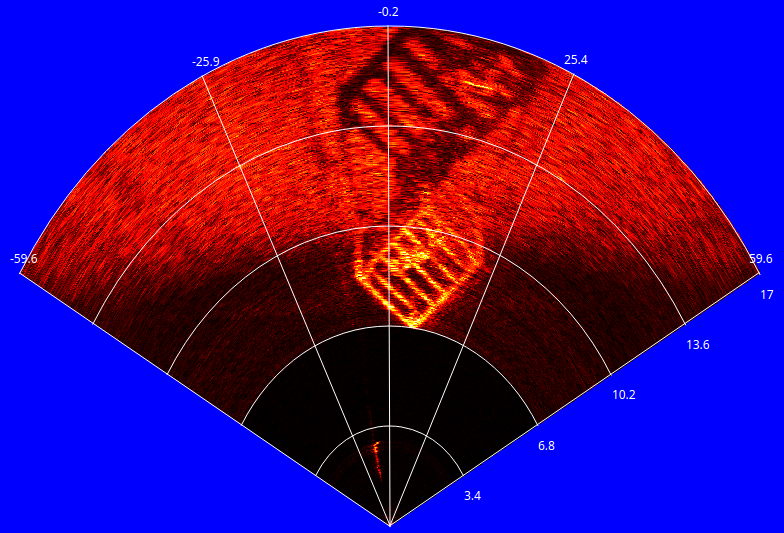
\includegraphics[width=0.4\paperwidth,height=6cm]{figs/eval_ssiv_real}
        \label{fig:eval:ssiv:real}
    }
    \setcounter{subfigure}{4}
    \subfigure[]{
        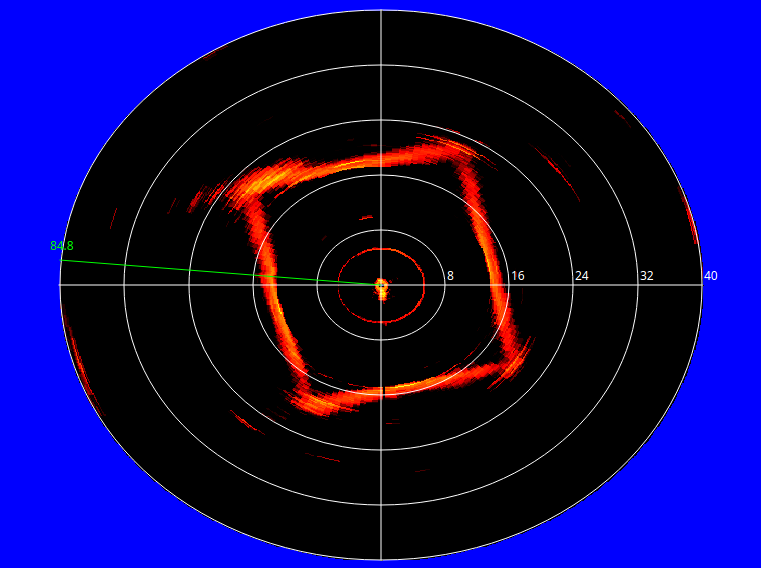
\includegraphics[width=0.4\paperwidth,height=6cm]{figs/eval_tank_real}
        \label{fig:eval:tank:real}
    }
    \setcounter{subfigure}{2}
    \subfigure[]{
        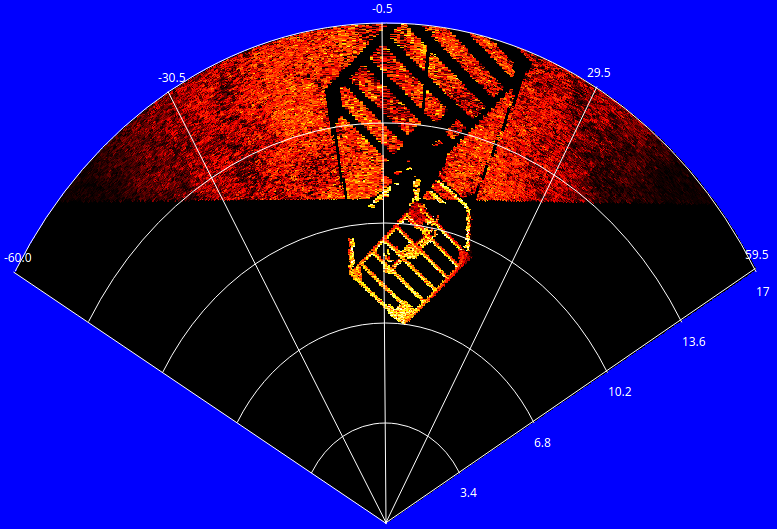
\includegraphics[width=0.4\paperwidth,height=6cm]{figs/eval_ssiv_sim}
        \label{fig:eval:ssiv:sim}
    }
    \setcounter{subfigure}{5}
    \subfigure[]{
        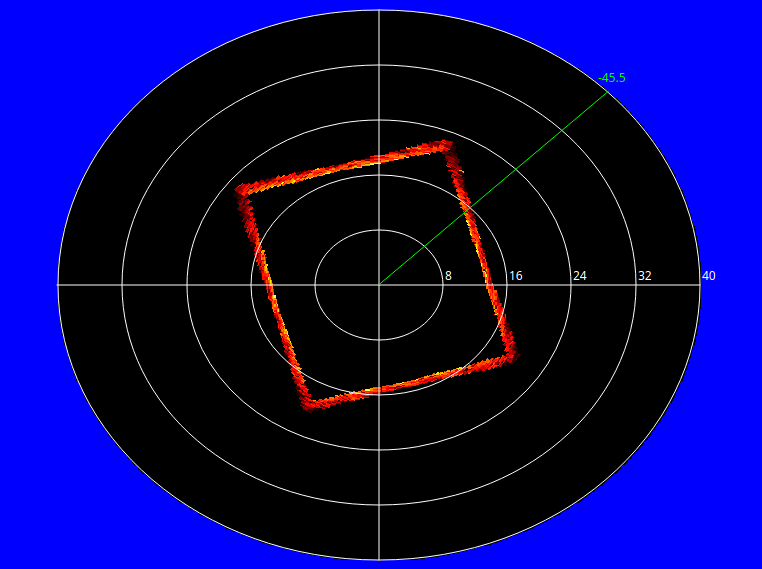
\includegraphics[width=0.4\paperwidth,height=6cm]{figs/eval_tank_sim}
        \label{fig:eval:tank:sim}
    }
    \captionsetup{justification=justified}
    \caption{\textcolor{blue}{Target objects used in the qualitative experimental evaluation: subsea isolation valve (SSIV) \subref{fig:eval:ssiv:photo} and big tank \subref{fig:eval:tank:photo}. Real-world sonar images and the virtual images generated by our approach, with the same device configurations: SSIV taken with Tritech Gemini 720i \subref{fig:eval:ssiv:real} and the corresponding simulated FLS image \subref{fig:eval:ssiv:sim}; tank walls taken with Tritech Micron DST \subref{fig:eval:tank:real} and the following simulated MSIS representation \subref{fig:eval:tank:sim}.}}
    \label{fig:eval}
\end{figure*}

\subsection{Computational time}

Performance evaluation of the simulator was assessed by considering the suitability to run real-time applications. The experiments were performed on a Intel Core i7 3540M processor, running at 3 GHz with 16GB DDR3 RAM memory and NVIDIA NVS 5200M video card, with Ubuntu 16.04 64 bits operating system. The elapsed time of each sonar data is stored to compute the average time, standard deviation and frame rate metrics, after $500$ iterations. The results found is summarized in Tables \ref{table:fls} and \ref{table:msis}. After changing the sonar rendering parameters, such as number of bins, number of beams and field-of-view, the proposed approach generated the sonar samples with a high
frame rate, for both sonar types, in comparison to real-world sonars. For instance, the Tritech Gemini 720i, a real forward-looking sonar sensor, with a field-of-view of $120^{\circ}$ by $20^{\circ}$ and 256 beams, presents a maximum update rate of 15 frames per second; so, the obtained results allow the use of the sonar simulator for real-time applications. Also, the MSIS produced data in the simulator is able to complete a $360^{\circ}$ scan sufficiently fast in comparison with a real sonar as Tritech Micron DST. For the FLS device, these rates are superior to the rates lists by DeMarco \textit{et al} \cite{demarco2015} ($330 ms$) and Saç \textit{et al} \cite{sac2015} ($2.5 min$). For MSIS type, to the best of our knowledge, there is no previous work for comparison.

According to previous results, since the number of bins is directly
proportional to sonar image resolution, we can conclude that the number of bins used affects the computational time; when the number of bins increases, the simulator will have a bigger scene frame to compute and to generate the sonar data.

\subsection{\textcolor{blue}{Quality evaluation of the simulated sonar image}}

\textcolor{blue}{Numerically assessing the performance of a sonar simulator is a non-trivial task. As sonar simulators are expected to work as trustworthy environment to avoid in-field experiments, the goal of quantitative evaluation should be to demonstrate that the real-world sonar image can be aligned with the synthetic one. Just two \cite{sac2015,demarco2015} out of the seven works analyzed in Section \ref{introduction} perform quantitative evaluation of the proposed simulators, although restricted only to computational time assessment.}

\textcolor{blue}{Similarity should be carried out by considering a real-world and a virtual scene, both insonified by real and virtual sonar devices, respectively, in the exact same conditions. In other words, it means that we have to guarantee the same poses of the AUV in the real and virtual scenarios, which, in turn, should present the same elements being insonified; measuring the alignment of the images (real and virtual) works as comparing how much the simulated sonar image is similar to the real one with respect to pixel intensity and location and image components.}

\textcolor{blue}{The process of measuring the image quality can be performed by a set of metrics, such as: mean-squared error (MSE), peak signal-to-noise ratio (PSNR), structural similarity index measure (SSIM), multi-scale structural similarity index measure (MS-SSIM), and interesting point detectors and distances (\textit{e.g.}, scale invariant feature transform - SIFT). To evaluate the quality of our approach, we attempted to model two real objects insonified by our AUV using FLS and MSIS, illustrated in Figs. \ref{fig:eval:ssiv:photo} and \ref{fig:eval:tank:photo}: a subsea isolation valve (SSIV) under the sea; and the big tank walls. Once the scenes were modeled, a pair of sonar images were produced: one from the real sonar device and another from the simulated sonar device, for each scene (Figs. \ref{fig:eval:ssiv:real}, \ref{fig:eval:ssiv:sim}, \ref{fig:eval:tank:real} and \ref{fig:eval:tank:sim}). After that, we applied the five aforementioned metrics to compute the degree of similarity between each pair of sonar images, presented in Table \ref{table:evaluation}.}

\textcolor{blue}{By the mathematical metrics (MSE and PSNR) results, based on pixel location and intensity differences, the simulated images presented a low error rate against the real images. Once the viewpoints in real and virtual scenes are approximated, the simulated images did not suffer from significant changes of insonified objects, as explained in Section \ref{sonar:characteristics}. Also, the additive noise in real images contains low intensity values, which did not interfere on these metrics evaluations.
The perceptual metrics (SSIM and MS-SSIM), based on human visual system, take into account visual attributes of images, such as luminance, contrast and structural terms. Since the tank scene has less insonified regions than the SSIV, and the FLS is more sensitive to the additive noise, the perceptual metrics results presented higher similarity for MSIS images than FLS.
By the end, the point-based methods do not work properly in noised images. So, it is expected that the SIFT presented low similarity results for both sonar devices.}

% \textcolor{blue}{Numerically assessing the performance of a sonar simulator is a non-trivial task. As sonar simulators is expected to work as trustworthy environment to avoid in-field experiments, the goal of the quantitative evaluation should be to demonstrating that the real-world sonar image can be aligned with the synthetic one. Just two \cite{sac2015,demarco2015} out of the seven works analyzed in Section \ref{introduction} perform quantitative evaluation of the proposed simulators, although restricted only to computational time assessment.}
%
% \textcolor{blue}{Image alignment (similarity) should be carried out by considering a real-world and a virtual scene, both insonified by real and virtual sonar devices, respectively, in the exact same conditions. In other words, it means that we have to guarantee the same poses of the AUV in the real and virtual scenarios, which, in turn, should present the same elements being insonified; measuring the alignment of the images (real and virtual) works as comparing how much the simulated sonar image is similar to the real one with respect to pixel intensity and location.}
%
% \textcolor{blue}{The process of measuring the alignment of two images can be performed by a set of measures, such as: mutual information (MI), mean-squared error (MSE), peak signal-to-noise ratio (PSNR), structural similarity index measure (SSIM), and interesting point detectors and distances (\textit{e.g.}, scale invariant feature transform - SIFT). To evaluate the alignment between the real and virtual images, we attempted to model two real scenes insonified by our AUV under the sea. Figure XX illustrated the two scenarios used to perform the evaluation. After the scenes were modeled, a pair of sonar images were produced: one from the real sonar device and another from the simulated sonar device, for each scene (see Figs. XX and XX). After that, we applied the five aforementioned alignment metrics to compute the degree of similarity between each pair of sonar images.}
%%% Colocar os resultados em tabelas
%%%Analisar os resultados:
%%% - Se forem bons: ótimo
%%% - Caso contrário, analisar a dificuldade do alinhamento por conta de não garantir a mesma "pose" dos AUVS nas cenas real e simulada - provavelmente deve ir por aqui. reforçar também que os outros trabalhos seguem pela linha de "human visual analysis para verificar o realismo e que as imagens de sonar dos trabalhos analisados não são "boas"

%%% Comentário de Rômulo: Resultados ruins das métricas podem ser explicados por problemas de: alinhamento, que implicam em mudanças de viewpoint e, consequentemente, shadows movements e mudanças significativas na representação acústica do objeto; atenuação do sinal; reverberação e interferências de fontes externas; além da simplificação do modelo 3d.

\begin{table}[t]
    \captionsetup{justification=justified}
    \caption{Similarity evaluation results between real-live and simulated sonar images.}
    \label{table:evaluation}
    \begin{center}
        \begin{tabular}{| c | c | c | c | c | c |}
            \hline
            \rule{0pt}{15pt}
            \makecell[c]{Scene} & \makecell[c]{\shortstack{MSE}} & \makecell[c]{\shortstack{PSNR}} & \makecell[c]{\shortstack{SSIM}} & \makecell[c]{\shortstack{MS-SSIM}} & \makecell{\shortstack{SIFT}}\\
            \hline
            SSIV & 0.01 & 20.002 & 0.361 & 0.654 & 4.19\% \\ \hline
            Tank & 0.01 & 23.787 & 0.834 & 0.895 & 28.8\% \\ \hline
        \end{tabular}
    \end{center}
\end{table}

% ----------------------------------------------------------------------------------

\section{Conclusion and future work}
\label{conclusion}

A GPU-based simulator for imaging sonar was proposed here. The system is able to reproduce the operation mode of two different types of sonar devices (FLS and MSIS) in real-time. The real sonar image singularities, such as multiplicative noise, surface properties and acoustic shadows are addressed, and represented in the simulated frames. Specially for the shadows, the acoustic representation can present information as useful as the insonified object. Considering the qualitative results, the sonar simulator can be used by feature detection algorithms, based on corners, lines and shapes. Also, the computational time to build one sonar frame was calculated using different device settings. The vertex and fragment processing during the underwater scene rendering accelerates the rendered sonar image, providing an average time close or better than real-world imaging devices. These results allow the use of this imaging sonar simulator by real-time applications, such as obstacle detection and avoidance, and object tracking. We are working now on a way to add the reverberation effect to perform a more close-to-real sensing, without significantly affecting the computational time. We are also working on how to include an additive noise in the simulation of the acoustic images. Future works will focus on qualitative and time consuming comparison with other sonar simulators.


% \nocite{*}
\bibliographystyle{model3-num-names}
\bibliography{elsarticle-template-3-num}

%% Authors are advised to submit their bibtex database files. They are
%% requested to list a bibtex style file in the manuscript if they do
%% not want to use model3-num-names.bst.

%% References without bibTeX database:

% \begin{thebibliography}{00}

%% \bibitem must have the following form:
%%   \bibitem{key}...
%%

% \bibitem{}

% \end{thebibliography}


\end{document}
